% DIAGNOSIS
%
% !TEX root = ../thesis-main.tex
%
\chapter{Diagnosis of lexical stress errors}
\label{chap:diagnosis}

%\cleanchapterquote{You can’t do better design with a computer, but you can speed up your work enormously.}{Wim Crouwel}{(Graphic designer and typographer)}

In order to provide learners with useful feedback on their lexical stress errors, % in the L2, 
a Computer-Assisted Pronunciation Training (CAPT) system
%the prototype CAPT tool developed in this thesis project 
must first be able to automatically detect and diagnose such errors in a learner's utterance. This requires at least:
\begin{enumerate}[label=(\alph*),topsep=-.5em]
\item Reasonably accurate word-, syllable- and phone-level segmentation of the learner's nonnative (L2) utterance; 
\item %A means of analyzing
An analysis of how lexical stress is realized in the
% prosody of the segmented 
given
utterance;
\item A representation of how native (L1) speakers of the target language (would) realize lexical stress in the given sentence; and
\item %A way of comparing
A comparison of the learner's prosody to this representation. 
\end{enumerate}

This chapter describes 
%
how (a) is achieved using
 forced-alignment segmentation of a learner's read-speech utterance with the corresponding text, 
 %and how problems in accuracy of the resulting segmentation can be overcome 
 (\cref{sec:diag:segmentation}); 
 %
 how the lexical stress analysis of (b), which is also crucial to (c), is produced by measuring the fundamental frequency, duration, and energy of relevant sections of the speech signal (\cref{sec:diag:prosody}); 
 %
 and 
 %finally, 
 the various approaches to (c) and (d) that are implemented in the prototype tool (\cref{sec:diag:compare,sec:diag:classification}).
 Finally, it describes how the system's modular architecture allows researchers and teachers control over which of these approaches are used (\cref{sec:diag:system}).



\section{Automatic segmentation of nonnative speech}
\label{sec:diag:segmentation}

%\TODO{Should this become a subsection of \cref{sec:diag:prosody}?}

%Automatic 
Segmentation
and labeling
of a recorded utterance is the task of annotating the speech signal with boundaries that demarcate individual phones, syllables, words, sentences, and/or other units of speech; see 
	\cref{fig:featuresexample} (\cpageref{fig:featuresexample})
	for examples of multi-level segmentations of word utterances from the IFCASL corpus (see \cref{sec:lexstress:data}).
	%\cref{fig:GGsegmentation} for an example of a multi-level segmentation of a German utterance. 
	
%	\begin{figure}
%		\centering
%		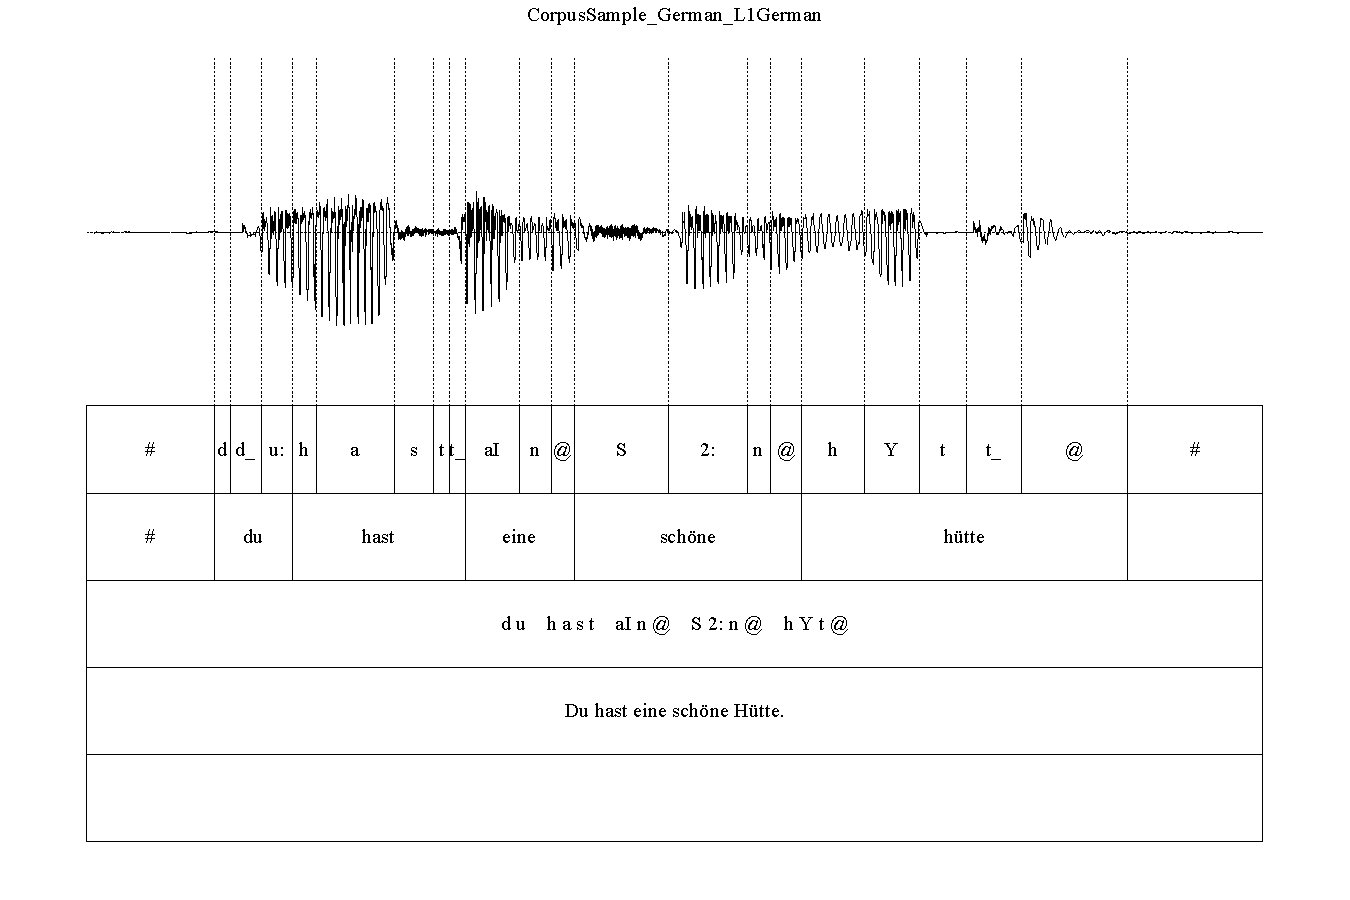
\includegraphics[width=\textwidth]{img/screenshots/SampleGG-basic}
%		\caption[An example German utterance and its segmentation]{\TODO{update with new example w/ SyllableTier} An example of a German utterance that has been segmented at the phone level (first row) and word level (second row). The third row contains the canonical (expected) native pronunciation of each word in the sentence, while the fourth row contains the written sentence of which the utterance is a reading.}
%		\label{fig:GGsegmentation}
%	\end{figure}


A reasonably accurate segmentation of an L2 learner's utterance is indispensable for an analysis of the accuracy of their pronunciation, 
%\TODO{mention that there are methods which don't need segmentation, but they're more limited?}
as it allows comparison between relevant units of the learner's utterance -- e.g. words, syllables, and phones -- and corresponding units in native speech. 
The most accurate segmentation would of course be one produced by hand by a trained phonetician; however, hand-labeling is not feasible in most scenarios because of its high cost in terms of time and wages. Moreover, because the ultimate goal of this work is the development of a CAPT tool which can give L2 learners helpful automatic feedback on their pronunciation, 
%even when they do not have access to a language teacher, 
any analysis of the learner's speech signal, including the preliminary step of segmentation, must proceed fully automatically. Therefore, a means of automatically segmenting a given utterance is required.



	%\subsection{Segmentation via forced alignment}
	%\label{sec:segmentation:alignment}
	
	When the content (text) of a given utterance is already known, the goal of automatic segmentation becomes aligning the  boundaries of each phone in the expected sentence with the appropriate points in the recorded signal. Boundaries for larger units such as syllables and words can be inferred from the phone boundaries. 
	An effective and widely-used technique for this is 
	forced
	% (Viterbi) 
	alignment \citep{Fohr1996,Mesbahi2011,Fohr2012,Fauth2014},
	a constrained type of speech recognition in which the task is not to determine what was said (i.e. the best phone or word sequence corresponding to a recorded utterance),  but rather to find the best alignment between the phone/word sequence, known in advance, and the corresponding segments of the given speech signal.
	%which uses the Viterbi algorithm to 
	%
	This technique	requires:
	\begin{itemize}[topsep=-1em]
%knowledge of the text of the given utterance (known beforehand in the IFCASL case), 
	\item the expected text (word sequence) of the given utterance, 
	\item a pronunciation lexicon containing the sequence of phones expected for each word, and
	\item an acoustic model for the target language.
	%which captures how phones in the target language (and potentially other phenomena, e.g. breathing or silence) are realized acoustically.
	\end{itemize}
	
	The first of these requirements, the text of the utterance, is trivial when the speaker has been asked to read a given sentence aloud, which is the case in this context.
	%
	A lexicon of canonical word pronunciations, i.e. the pronunciations that might be given in a standard dictionary, is also relatively easy to obtain for a well-researched language such as German, for which many digital linguistic resources exist; one example is the lexicon of the MARY text-to-speech synthesis system \citep{Schroeder2003}.
	 To account for differences in how different speakers (especially nonnative speakers) may pronounce the given sentence, 
	%the lexicon is supplemented with a lexicon of nonnative pronunciation variants 
	the lexicon should contain not only the canonical pronunciation for each word, but also any alternate or non-standard pronunciation variants (native or nonnative) that might be encountered. As stated in \cref{sec:capt:auto} researchers at LORIA have found the inclusion of nonnative pronunciation variants to lead to improvements in the accuracy of automatic segmentation of nonnative speech \citep{Jouvet2011,Mesbahi2011,Bonneau2012,Orosanu2012}.
	%and the IFCASL corpus has been segmented using model
	%and one of the intended outcomes of the IFCASL project is the extraction of a nonnative variant lexicon from the L2 speech in the corpus \TODO{ref?}.
	
	The final requirement for segmentation via forced alignment is an acoustic model, i.e. a statistical model 
	%(typically a Hidden Markov Model) 
	%trained on speech in the target language 
	which captures the correspondence between acoustic features extracted from the speech signal and phones in the target language. 
	To accurately capture this correspondence, the model must be trained on a large amount of speech data in the target language; 
	the acoustic model used to align the German IFCASL data was trained on native German speech from the Kiel corpus \citep{Kohler1996}.
	However, research by \textcite{Bouselmi2005,Bouselmi2012} 	
	%\citeauthor{Bouselmi2005} (\citeyear{Bouselmi2005,Bouselmi2012}) 
	has shown that even more accurate segmentation of learners' utterances can be obtained by using acoustic models adapted to L2 speech in the target language and/or speech in the learner's L1; refining the automatic segmentation functionality using such adapted models would therefore be a logical extension of this work.
	%\TODO{\textit{remove} (see \cref{sec:conclusion:future})}. % \TODO{does that clause work?}.
	
	%\TODO{Details about how forced Viterbi alignment works?}
	%Given the expected text and the corresponding phone sequence, forced alignment consists of using the Viterbi algorithm and an acoustic Hidden Markov Model trained on the target language to determine the temporal locations of boundaries between each of the expected phones. The Viterbi algorithm is commonly used in automatic speech recognition to determine... 

	
	Given these resources, the JSnoori software,
	which \TODO{de-stress} uses for speech processing,
	%used to process speech in the lexical stress CAPT tool
	is capable of automatically segmenting a learner's utterance almost instantly. 
	%Unfortunately, a disadvantage of forced alignment is that it requires the entire utterance (e.g. sentence), so real-time segmentation is not possible \TODO{true? should this go in a footnote?}. 
	However, acoustic models and pronunciation lexicons for German have yet to be integrated into JSnoori, which 
	%is currently only capable of segmenting 
	currently only has the resources to segment 
	speech in English and French.
	 %In the absence of automatic segmentation capabilities for German,
	 Therefore,
	 In its current implementation, \TODO{de-stress}
	 presupposes the existence of a segmentation for a given utterance,
	%the tool %thus takes 
	taking a ``Wizard-of-Oz'' approach to the automatic segmentation step by demonstrating its error diagnosis and feedback capabilities using learner (L2) and reference (L1) read-speech utterances from the German-language subset of the IFCASL corpus \citep{Fauth2014,Trouvain2013}, all of which have been segmented at the phone and word levels using the forced alignment technique described above.
	Once the requisite German-language resources are available in JSnoori, \TODO{de-stress} can easily be extended to perform on-the-fly segmentation of learner utterances. % (see \cref{sec:conclusion:future}).
	
	%\TODO{a real CAPT system would have to do this on the fly, and that can be done in JSnoori, but the prototype assumes segmentation has been done and mocks that up by only using auto segmentations of IFCASL data}
	%
	
	
	Although the IFCASL corpus also contains manually-corrected versions of the majority of the forced-alignment segmentations,
	\TODO{de-stress} only makes use of the automatically-determined determined boundaries, even though these are potentially less accurate; 
	this is to more accurately 
	%reflect the fact that any 
	simulate the conditions of a 
	fully-fledged CAPT system,
	which 
	would need to perform segmentation on the fly without recourse to manual verification.
	%The native and nonnative read speech recordings comprising the German-language subset of the IFCASL corpus \citep{Fauth2014,Trouvain2013} have already been automatically segmented via forced alignment, as described above.
	%\TODO{paragraph break?}
	Indeed, 
	%segmentations obtained by forced alignment 
	forced alignment is not a perfect method; because of the constraints put on the recognition system, it will always find a match between the given text and audio, even if they do not correspond (e.g. if a completely different sentence/word was uttered).  
	Therefore, inaccuracies in the phone boundaries determined using this technique must be expected, especially when the alignment is performed on nonnative utterances using an acoustic model trained on native speech.
	As discussed in \cref{sec:capt:auto}, however, \textcite{Mesbahi2011} compared manual segmentations of L2 speech with automatic segmentations produced via these techniques, and concluded that the automatically-produced segment boundaries were accurate enough to be useful in CAPT for prosodic feedback.
		Nonetheless, a fully-fledged CAPT system extending \TODO{de-stress} would ultimately have to cope with any problems that may result from using imperfect automatic segmentations as a starting point for analysis; this could be accomplished using techniques for detecting incorrect utterances such as those developed by \textcite{Bonneau2012,Orosanu2012}, as discussed in \cref{sec:capt:auto}.
	
	
	As mentioned above, the utterances in the IFCASL corpus have %pre-existing 
	segmentations at the phone and word levels; however, the corpus does not contain syllable-level segmentations.
	%but not at the syllable level.
	%and a subset of these automatic segmentations has been manually verified.
	%As the syllable is arguably the most important unit for analysis of lexical stress realization \TODO{reference/justification},
	As syllable-level analysis is important for the diagnosis of lexical stress errors, syllable segmentations had to be created for each utterance. This was accomplished by 
	 %However, segmentation at the syllable level still needs to be performed. This may be accomplished based on the word- and phone-level annotations by automatically or 
	 manually determining the locations of syllable boundaries in the phone sequence for each word, 		%(i.e. the locations in the phone sequence where syllable boundaries are expected) 
	 %using the text of each sentence and a syllabified phonetic lexicon from the speech synthesis system MaryTTS \citep{Schroeder2003}, 
	%\TODO{using the syllabification program [...] and a pronunciation dictionary?  },
	 %Given the sequence of phones expected for each syllable, the locations of syllable boundaries were automatically extracted 
	 %using  to 
	 automatically extracting the temporal locations of these %syllable 
	 boundaries
	 from the phone-level segmentation, 
	 and automatically combining the word-internal syllable boundaries with the boundaries in the word-level segmentation to create the syllable-level segmentation. 


	

	
%%%%%%%%%%%%%%%%%%%%%%%
%%% Moved to Future Work
%%%%%%%%%%%%%%%%%%%%%%%
	%\subsection{Evaluation of segmentation accuracy}
	%\label{sec:segmentation:eval}
%	
%	The accuracy of the forced-alignment segmentation can be assessed by computing inter-annotator agreement between the automatically produced segmentation and one or more manually-verified segmentations. The team at LORIA in Nancy has already completed this evaluation for the French IFCASL sub-corpus using the CoALT tool \citep{Fohr2012}. In cooperation with that team, the German sub-corpus (or a subset thereof) will be evaluated in the same way.
%	A similar evaluation will be carried out for the syllable-level segmentations, a subset of which will be manually verified.
%
%%	Error analysis will be performed for each boundary type, to enable identification of the types of boundaries at which the system tends (not) to make many errors. This detailed analysis will contribute to error management in the system, as described 
%%in \cref{sec:segmentation:errors}.
%%below.

%	\subsection{Coping with segmentation errors}
%	\label{sec:segmentation:errors}
%	
%	Forced alignment is not a perfect method; because of the constraints put on the recognition system, the aligner will always find a match between the given text and audio, even if they do not correspond. Incorrect segmentation can lead to mistakes in diagnosis, so CAPT systems must have a means of reducing, or at least monitoring, the amount of error introduced by inaccurate segmentation \citep{Eskenazi2009}. 	
%	In the proposed CAPT tool, this function may be served by the development of a simple sentence- and/or word-level confidence measure. 
%	While it is very difficult to compute such a measure directly from the decoding scores of the forced aligner, it may be possible to determine from the aforementioned accuracy evaluation which types of boundaries (e.g. between a sonorant and a vowel) the aligner typically has trouble detecting accurately, and then to calculate, for a given utterance, the proportion of error-prone boundaries. While a very simplistic measure, this could nevertheless provide some indication of when (not) to trust the automatic alignment, thus impacting decisions on how and whether to attempt error diagnosis (or feedback).
%	% based on the boundary error rates found in \cref{sec:segmentation:eval}. 
%	Other error-management strategies may also be explored, such as the type of error-filtering methods described by \textcite{Mesbahi2011,Bonneau2012,Orosanu2012}, in which utterances which do not correspond to the expected text are detected and rejected before alignment is attempted.
%%%%%%%%%%%%%%%%%%%%%%%
	
\section{Analysis of word prosody}
\label{sec:diag:prosody}

	%\TODO{Technically these features aren't all relevant to comparison-based diagnosis, only classification - so I guess this whole section needs to be rewritten :/}
	
	The automatically-determined word, syllable, and phone boundaries obtained as described in the previous section 
	%were used to 
	enable the CAPT tool to locate and analyze segments of the speech signal relevant to the realization of lexical stress.
	%, enabling analysis of these  
	%in terms of the acoustic correlates of word prosody described in \cref{sec:background:stress}.  
	This section describes the features by which the system analyzes the lexical stress prosody of an utterance, be it the utterance of a learner or of a native speaker. These features relate to the three acoustic properties (and by extension their perceptual correlates) described in \cref{sec:bkgd:stress}, namely duration (timing), fundamental frequency (pitch), and intensity (loudness). 
	The relative utility of these features in automatically diagnosing lexical stress errors is discussed further in \cref{sec:diag:classification}.
		%The features computed for each property are described in the corresponding sections below.
%
	%\TODO{Where possible, the diagnosis module of the CAPT tool will provide researchers control over the features used; for example, there may be an option to include all F0 and duration features but ignore intensity features.}
%	

%TODO {\textit{To go somewhere in this section:} Added German phonetic inventories to JSnoori so that it could know e.g. which segments are vowels}


	Throughout this section, the features discussed are illustrated with their values for a word from two sample utterances of a German word selected from the IFCASL corpus:
	one by a native German speaker (assumed to represent a correct realization of lexical stress), the other an utterance from an L1 French speaker which was assigned a gold-standard label of [incorrect] (see \cref{chap:lexstress}).
%one by a L1 French speaker and the other by a L1 German speaker.
 The oscillogram, waveform, and segmentations for these samples are shown in \cref{fig:featuresexample}.
	
	\begin{figure}
		\centering
		
		 \begin{subfigure}{\textwidth}
                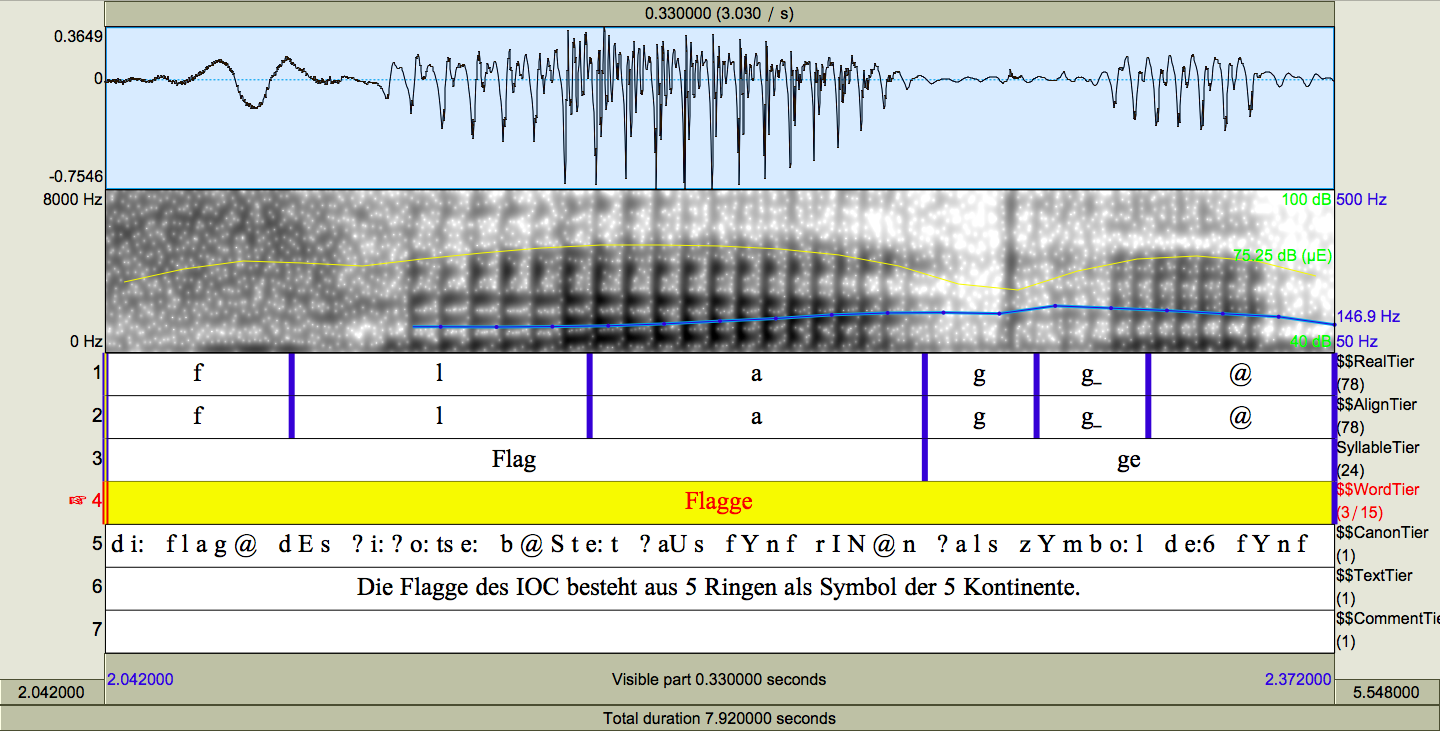
\includegraphics[width=\textwidth]{img/screenshots/2SH05_GGMB2_035-flagge}
                \caption{L1 German speaker (G)}
                \label{fig:featuresexample:gg}
        \end{subfigure}%
        
        \vspace{1.5em}

        
		\begin{subfigure}{\textwidth}
                %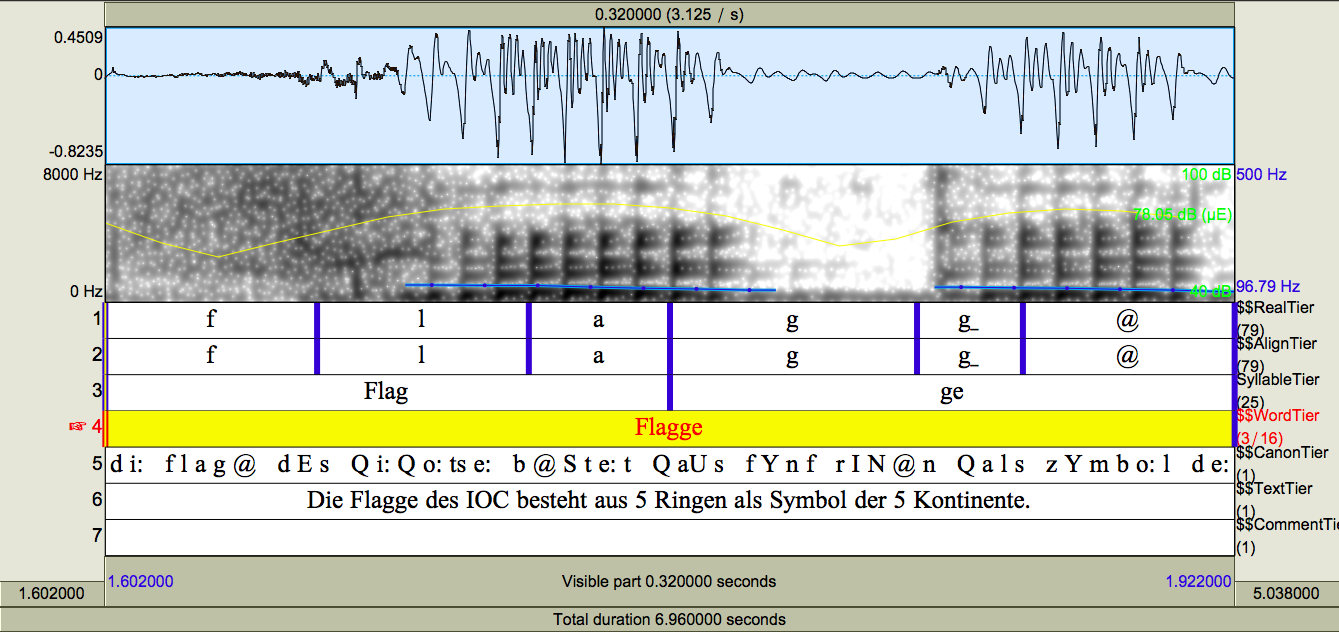
\includegraphics[width=\textwidth]{img/screenshots/2SH05_FGMB1_527-flagge}
                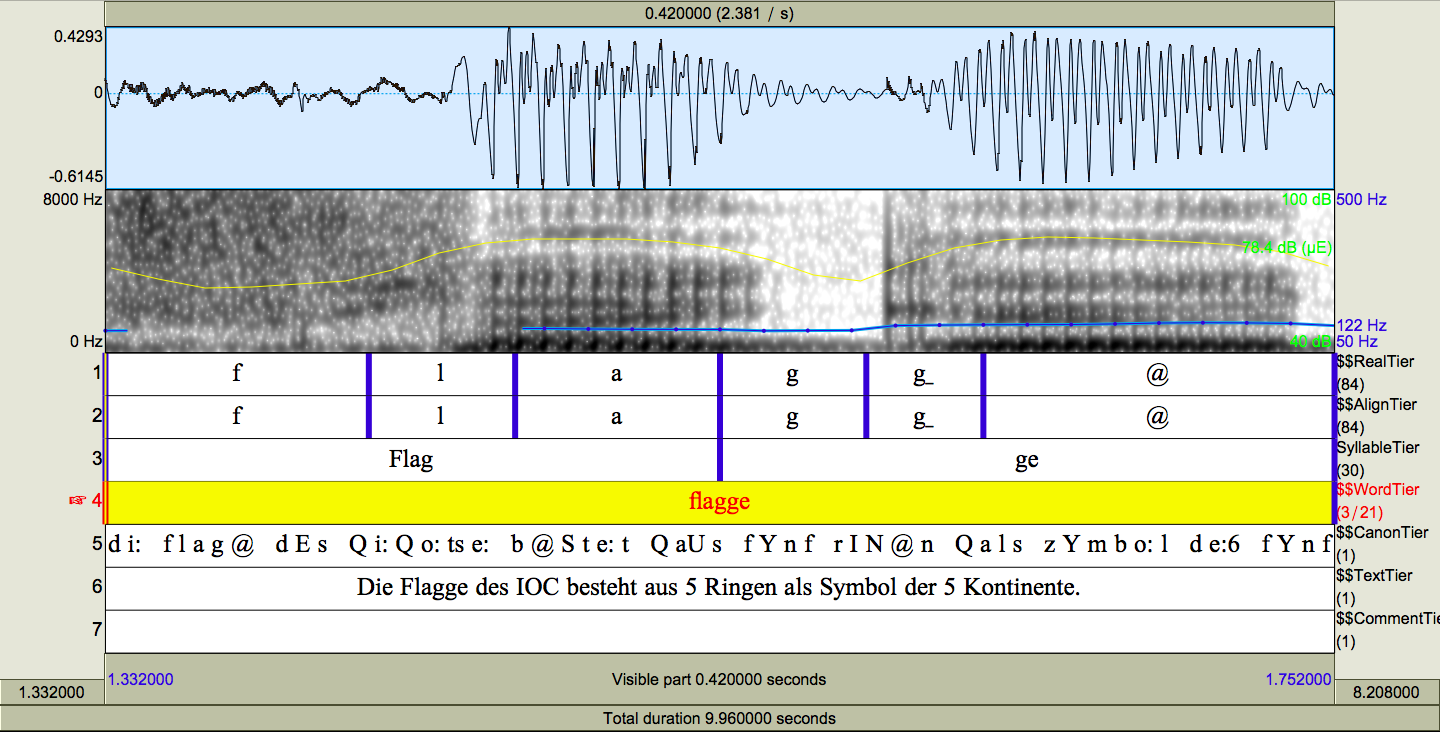
\includegraphics[width=\textwidth]{img/screenshots/2SH05_FGMA2_526-flagge}
                \caption{L1 French speaker (F)}
                \label{fig:featuresexample:fg}
        \end{subfigure}%
        
        \vspace{1.5em}

		\caption[Sample L1 and L2 word utterances]{Two sample utterances of the word "Flagge" from the IFCASL corpus, used to illustrate the features discussed in this section. In these Praat screenshots, the oscillogram and spectrogram of the signal are visible in the top portion of the image, while the bottom portion displays the corresponding segmentations. Segmentations at the phone, syllable, and word level are displayed, along with the canonical phone sequence and orthographic form of the uttered sentence.}
		\label{fig:featuresexample}
	\end{figure}
	
Once again it should be stressed that the features described below are computed from the automatically generated segmentation of a given utterance, and not from a hand-corrected segmentation; as a result, the computed values may be slightly (or in some cases, significantly) inaccurate due to errors in the forced-alignment segmentation process, as just discussed in \cref{sec:diag:segmentation}. %MOVED ABOVE This reliance only on automatically-detected segment boundaries is intentional, as it simulates the conditions of an automatic, real-time tutoring system, which would need to perform segmentation on the fly and would not have recourse to human verification of segment boundary locations.
	%
	%\TODO{\textit{Worth mentioning? Seems a bit out of place}} 
	%A potential complication of this analysis that should be pointed out relates to 
	Another potential complication worth noting is the fact that we are here dealing exclusively with read, and not spontaneous, speech. As \textcite[p.~275]{Cutler2005} remarks, ``acoustic differences between stressed and unstressed syllables are relatively large in spontaneous speech. With laboratory-read materials, however, such differences do not always arise.'' Therefore, the task of recognizing prosodic deviations in learners' read speech may be somewhat different than the corresponding task for spontaneous speech, and this difference should be kept in mind in the discussion that follows.

	\subsection{Duration}
	\label{sec:prosody:duration}

	Analysis of duration (timing) is extremely important for detecting stress patterns;
indeed, some research indicates that syllable duration may be the most important, if not the only acoustic correlate of lexical stress in German (e.g. \cite{Dogil1999}).
%as discussed in section \cref{sec:stress:german} above.}
%In this work, duration analysis will figure prominently, and following \textcite{Bonneau2011} will most likely take into account the relative duration of each syllable of the word in question, and/or of the vowel at the nucleus of each syllable. %Other features may also be explored.
Duration analysis therefore figures prominently in the analysis and assessment of learners' lexical stress in this work. 


Given the word-, syllable- and phone-level segmentations of an utterance (see \cref{sec:diag:segmentation}), the extraction of duration features for that utterance is trivial, as it consists simply of noting the duration of each relevant segment. % in the appropriate segmentation. 
Following \textcite{Bonneau2011}, duration analysis in this work takes into account the %relative
 duration of each syllable in the word to be analyzed, and
 %as well as the %relative duration 
 of the vowels at the nucleus of each syllable. 
 	%\TODO{Mention that to find vowels I had to add German phonetic inventory to JSnoori?}
	To account for inter-speaker variability, e.g. the fact that some speakers may have an overall slower or faster speech rate than others, relative rather than absolute durations are used.
	The list of duration features computed for each word utterance is given in \cref{tab:durationfeatures}, 
along with the values computed for each feature from the sample utterances shown in \cref{fig:featuresexample}. % from the IFCASL corpus \TODO{reference?}. 


\begin{table}%[ht]
		\centering
		\caption[Features used for duration analysis]{Features used for duration analysis, and their values for the sample utterances of ``Flagge'' in \cref{fig:featuresexample}. 
		S0 refers to the word's first syllable, S1 to the second syllable; similarly, V0 and V1 refer to the nucleus (vowel) of the first and second syllable, respectively.
		}
		
%		\begin{subtable}[h]{\textwidth}
%		\caption{Absolute features}
%		\begin{tabularx}{\textwidth}{lXcc}
%		\toprule
%		\multirow{2}{*}{Feature name} 
%									& \multirow{2}{*}{Description}
%																	& \multicolumn{2}{c}{Value (seconds)} \\
%					  				&												&  (a) F		& (b) G \\
%		\midrule
%		WORD-DUR 		&	Duration of entire word \TODO{remove?}				& 0.32			& 0.33			\\
%		SYLL0-DUR 		&	Dur. of 1st syllable						& 0.16			& 0.22			\\
%		SYLL1-DUR 		&	Dur. of 2nd syllable				& 0.16			& 0.11			\\
%		V0-DUR 				&	Dur. of vowel in 1st syllable		& 0.04			& 0.09			\\
%		V1-DUR 				&	Dur. of vowel in 2nd syllable	& 0.06			& 0.05			\\
%		\bottomrule
%		\end{tabularx}
%		\end{subtable}
%
%		\vspace{1em}		
%		
%		\begin{subtable}[h]{\textwidth}
%		\caption{Relative features}
		\begin{tabularx}{\textwidth}{lXcc}
		\toprule
		\multirow{2}{*}{Feature name} 
									& \multirow{2}{*}{Description}
														& \multicolumn{2}{c}{Value} \\
	&												&  (a) G		& (b) F \\
		\midrule
		REL-SYLL-DUR 	
			& Duration of S1$/$duration of S0
			%&	SYLL1-DUR$/$SYLL0-DUR 		
			& 	0.50		& 	1.00	\\
		REL-V-DUR 		
			& Duration of V1$/$duration of V0
			%&	V1-DUR$/$V0-DUR					
			& 	0.56		& 	1.71	\\
		\bottomrule	
		\end{tabularx}
%		\end{subtable}
		\label{tab:durationfeatures}
\end{table}



	\subsection{Fundamental frequency}
	\label{sec:prosody:f0}
	
	
	As described in \cref{sec:bkgd:stress}, the fundamental frequency (F0) of an utterance, which corresponds at the perceptual level to its pitch, also provides a strong indication of how lexical stress is realized in that utterance, and F0 features 
	%should therefore also contribute to 
	are another crucial component of
	the system's prosodic analysis. 
	%
	
%		\TODO{Pitch in JSnoori:
%	\begin{itemize}
%		%\item Martin's basic spectral comb algo
%		\item Yves' improvement using parabolic interpolation
%		%\item Secrest \& Doddington's improvement for voicing decision 
%		%\item dynamic programming (Ney?) to select which F0 values to accept
%		\item Soon to implement Yin temporal method, and then combine results with those of Martin's or another spectral method such as SWIPE (SWYPE?) (combining with NNs or something else)
%		%\item semitones
%		%\item 0 values are excluded from mean calculations
%	\end{itemize}	
%	}	
	
	The pitch (F0)%
	\footnote{ As stated previously, pitch and F0 are not identical, 
	the latter being an acoustic (objective) property of the speech signal and the former the perceptual (subjective) correlate thereof. 
	However, in JSnoori and much of the literature, the term ``pitch'' is often used to refer to an aspect of the speech signal which can be measured objectively.
	For consistency with JSnoori's terminology, in this section the terms will be used somewhat interchageably.}
	 contour of a given utterance is estimated using the pitch detection 
	%algorithm(s) implemented in 
	functionality of 
	JSnoori. At the heart of JSnoori's approach to pitch detection lies the algorithm developed by \textcite{Martin1982}, a frequency-domain method of pitch detection which uses a comb function with teeth of decreasing magnitude to identify harmonics of F0 in the spectrum (spectra are extracted by Fast Fourier Transform using 32-millisecond Hamming windows offset by 8 milliseconds). JSnoori also implements several improvements to pitch detection beyond Martin's algorithm \citep{DiMartino1999}, including
	 %\TODO{Yves' parabolic interpolation - citation?}, 
	 the voicing decision optimization of   \textcite{Secrest1983} 
	 and the dynamic programming technique proposed by \textcite{Ney1981} for identifying and removing incorrect points in the contour. 
	 %Further improvements to JSnoori's pitch detection capabilities, including the implementation of additional detection algorithms, are currently in development (see \cref{sec:conclusion:future}).
	
	Thanks to these techniques, JSnoori is capable of efficient, generally accurate detection of F0 
	within the range of 65-800 Hertz (Hz), with each pitch point in the contour being subsequently converted from Hz to semitones.
	%, using the Bagshaw definition \citep{Bagshaw1994} (or \citep{Bonneau2004}?)
	Using this contour, each of the relevant segments of the utterance -- i.e. the word of interest, each of its syllables, and their nuclei -- is analyzed in terms of its F0 mean, maximum, minimum, and range;
	the full list of features computed is presented in \cref{tab:f0features}.
	Features only take into account the non-zero points in the contour, i.e. points corresponding to voiced sections of the utterance. The F0 mean is calculated as the average of all non-zero points within the start and end boundaries of the given segment; the maximum F0 is the highest value at any of these points, and the minimum the lowest non-zero value; and F0 range is computed as the difference between the maximum and minimum values. 
	
	%\TODO{JSnoori only looks at mean and max? or something? by way of transition to this next paragraph}
	% JSnoori diagnoses errors in the learner's pitch only with regard to 
	
	Much of the work on assessing nonnative lexical stress has been conducted with English as the L2, and thus often makes the assumption that a stressed syllable should have a higher F0 than unstressed syllables \citep{Bonneau2011}. In German, the F0 of a stressed syllable also tends to differ from the surrounding contour, but the difference may be positive (the stressed syllable has a higher pitch than surrounding syllables) or negative (lower pitch) \citep[p.~267]{Cutler2005}. 		%``...in German utterances, stressed syllables could be signaled by any F0 obtrusion from the overall contour, so that a stressed syllable could be either higher or lower in pitch than its neighbors'' \citep[p.~267]{Cutler2005}
	Therefore, the computed features
	%include not only the difference in F0 maxima between syllables in the word and the location (syllable index) of the word's F0 maximum, but also the analogous features for F0 minima and ranges.
	capture not only the F0 maximum of each syllable, but also the minimum and range (difference between maximum and minimum). %\TODO{more/separate discussion of why range might be important?}.
	 
	%To guard against unvoiced segments interfering with the F0 analysis, syllables may be represented by the vowels that form their nuclei. Relative differences between syllables may be more helpful than absolute differences. The F0 variation (range) over the entire word might also be informative of whether or not the speaker failed to stress any syllable.%, although it would not tell us which syllable were stressed. 
	%Other features may be drawn from related work on lexical stress in learner speech, such as \textcite{Bonneau2011}.
	


%		%\setlength\extrarowheight{5pt}
%\begin{table}[h!]
%		\centering
%		\caption[Features used for fundamental frequency (F0) analysis]{Features used for fundamental frequency (F0) analysis, and their values for the sample utterances of ``Flagge'' in \cref{fig:featuresexample}.% Values are given in semitones.
%		}
%		{\renewcommand{\arraystretch}{1.25}%
%		
%		\begin{subtable}[h]{\textwidth}
%		\caption{Absolute features}
%		\begin{tabularx}{\textwidth}{p{.225\textwidth}Xrr}
%		\toprule
%		\multirow{3}{*}{Feature name} 
%									& \multirow{3}{*}{Description}
%																	& \multicolumn{2}{c}{Value} \\
%									&								& \multicolumn{2}{c}{(semitones)} \\							
%					  				&																	&  (a) F		
%					  																											& (b) G
%					  																																\\
%		\midrule
%		%%%% WORD FEATURES 
%		WORD-F0-MEAN	& Average (Avg.) F0, entire word	 				& 8.78		& 16.36\\
%		WORD-F0-MAX	& Maximum (Max.) F0, entire word				& 10.73	& 20.08\\
%		WORD-F0-MIN		& Minimum (Min.) F0, entire word				& 6.27		& 13.65\\
%		WORD-F0-RANGE & WORD-F0-MAX$-$WORD-F0-MIN			& 4.46		& 6.43\\
%%		WORD-F0-RANGE & {\renewcommand{\arraystretch}{.9}%
%%										$\displaystyle\begin{array}{l}%
%%										\phantom{-}\mbox{WORD-F0-MAX}\\%
%%										-\mbox{WORD-F0-MIN}\\\end{array}$}	& 4.46	& 6.43\\
%%		\multirow{2}{*}{WORD-F0-RANGE}	
%%									& $\phantom{- }\text{WORD-F0-MAX}$
%%																			& \multirow{2}{*}{4.459217}		
%%																									& \multirow{2}{*}{6.425775}\\
%%									& $- \text{WORD-F0-MIN}$						& 						& 					\\		
%
%		%\addlinespace
%		%%%% SYLL* FEATURES 
%		SYLL0-F0-MEAN	& Avg. F0, 1st syllable					& 9.29		& 15.81\\	
%		V0-F0-MEAN		& Avg. F0, 1st syllable	nucleus				& \color{red}{TD}		& \color{red}{TD}\\
%		SYLL0-F0-MAX		& Max. F0, 1st syllable					& 10.73		& 18.25\\
%		V0-F0-MAX		& Max. F0, 1st syllable	nucleus				& \color{red}{TD}		& \color{red}{TD}\\
%		SYLL0-F0-MIN		& Min. F0, 1st syllable					& \color{red}{TD}		& \color{red}{TD}\\
%		V0-F0-MIN		& Min. F0, 1st syllable	nucleus				& \color{red}{TD}		& \color{red}{TD}\\
%		SYLL0-F0-RANGE & SYLL0-F0-MAX$-$SYLL0-F0-MIN	& 1.45		& 4.60\\
%		V0-F0-RANGE		& V0-F0-MAX$-$V0-F0-MIN				& \color{red}{TD}		& \color{red}{TD}\\
%%		SYLL0-F0-RANGE	& {\renewcommand{\arraystretch}{.9}%
%%										$\displaystyle\begin{array}{l}%
%%										\phantom{-}\mbox{SYLL0-F0-MAX}\\%
%%										-\mbox{SYLL0-F0-MIN}\\\end{array}$} 		& 1.45		& 4.60\\
%%		\multirow{2}{*}{SYLL0-F0-RANGE}	
%%									& $\phantom{- }\text{SYLL0-F0-MAX}$%-$SYLL0-F0-MIN	
%%																			& \multirow{2}{*}{1.44952}		
%%																										& \multirow{2}{*}{4.600318}\\
%%									& $- \text{SYLL0-F0-MIN}$					& 						& 					\\		
%
%		SYLL1-F0-MEAN	& Avg. F0, 2nd syllable						& 8.24		& 17.51\\
%		V1-F0-MEAN		& Avg. F0, 2nd syllable	nucleus				& \color{red}{TD}		& \color{red}{TD}\\
%		SYLL1-F0-MAX		& Max. F0, 2nd syllable						& 9.93		& 20.08\\
%		V1-F0-MAX		& Max. F0, 2nd syllable	nucleus				& \color{red}{TD}		& \color{red}{TD}\\
%		SYLL1-F0-MIN		& Min. F0, 2nd syllable			& \color{red}{TD}	& \color{red}{TD}\\
%		V1-F0-MIN		& Min. F0, 2nd syllable 	nucleus				& \color{red}{TD}		& \color{red}{TD}\\
%		SYLL1-F0-RANGE	& SYLL1-F0-MAX$-$SYLL1-F0-MIN 	& 3.66		& 5.86 \\
%		V1-F0-RANGE		& V1-F0-MAX$-$V1-F0-MIN				& \color{red}{TD}		& \color{red}{TD}\\
%%		SYLL1-F0-RANGE	& {\renewcommand{\arraystretch}{.9}%
%%										$\displaystyle\begin{array}{l}%
%%										\phantom{-}\mbox{SYLL1-F0-MAX}\\%
%%										-\mbox{SYLL1-F0-MIN}\\\end{array}$} 		& 3.66	& 5.86 \\
%%		\multirow{2}{*}{SYLL1-F0-RANGE}	
%%									& $\phantom{- }\text{SYLL1-F0-MAX}$%-$SYLL1-F0-MIN	
%%																			& \multirow{2}{*}{3.65978}		
%%																										& \multirow{2}{*}{5.862722}\\
%%									& $- \text{SYLL1-F0-MIN}$					& 						& 					\\		
%		
%		%\addlinespace
%		\bottomrule
%		\end{tabularx}
%		\end{subtable}
%		}
%		\label{tab:f0features}
%		\end{table}
%		%\vspace{1em}
		
		\begin{table}%[h!]
		
		%\ContinuedFloat
		\caption[Features used for fundamental frequency (F0) analysis% (cont.)
		]{%(continued) 
		Features used for fundamental frequency (F0) analysis, and their values for the sample utterances of ``Flagge'' in \cref{fig:featuresexample}. 
		S0 refers to the word's first syllable, S1 to the second syllable; similarly, V0 and V1 refer to the nucleus (vowel) of the first and second syllable, respectively.
		}
		{\renewcommand{\arraystretch}{1.25}%
		%\begin{subtable}[h]{\textwidth}
		%\caption{Relative features}
		\begin{tabularx}{\textwidth}%{p{.25\textwidth}Xrr}
			{lXrr}
		\toprule
		\multirow{2}{*}{Feature name} 
									& \multirow{2}{*}{Description}
													& \multicolumn{2}{c}{Value} \\						
					  				&							&  (a) G		& (b) F
					  																																\\
		\midrule
		%%%% RELATIVE FEATURES 
%		SYLL-REL-MEAN & {\renewcommand{\arraystretch}{.9}%
%									 $\displaystyle\begin{array}{l}
%									 \mbox{SYLL0-F0-MEAN}\\
%									 \hline
%									 \mbox{SYLL1-F0-MEAN}\\
%									 \end{array}$}			
%																				& 1.12688     & 0.903218 \\		
		REL-SYLL-F0-MEAN 
			& Mean F0 in S1$/$mean F0 in S0
			%& Mean F0 in 2nd syllable$/$mean F0, 1st syll.
			%& SYLL0-F0-MEAN$/$SYLL1-F0-MEAN 	
			& 1.11    & 1.09 \\
			
		REL-V-F0-MEAN 
			& Mean F0 in V1$/$mean F0 in V0
			%& Mean F0, 2nd syll. nucleus$/$mean F0,1st syll. nuc.
			%& V1-F0-MEAN$/$V0-F0-MEAN 
			&  0.95		& 1.10 \\
%		SYLL-REL-MEAN
%							& $\displaystyle\frac{\mbox{SYLL0-F0-MEAN}}{\mbox{SYLL1-F0-MEAN}}$			
%																									& 1.13    & 0.90 \\
		%\addlinespace
		
		REL-SYLL-F0-MAX 
			& Maximum F0 in S1$/$max. F0 in S0
			%& SYLL1-F0-MAX$/$SYLL0-F0-MAX 			
			& 1.10    & 1.12 \\
			
		REL-V-F0-MAX 
			& Max. F0 in V1$/$max. F0 in V0
			%& V1-F0-MAX$/$V0-F0-MAX 
			&  0.96	& 1.12\\
%		SYLL-REL-MAX
%							& $\displaystyle\frac{\mbox{SYLL0-F0-MAX}}{\mbox{SYLL1-F0-MAX}}$
%																									& 1.08		& 0.91 \\

		REL-SYLL-F0-MIN 
			& Minimum F0 ($>0$) in S1$/$min. F0 in S0
			%& SYLL1-F0-MIN$/$SYLL0-F0-MIN 
			&	1.04		&	1.04	\\
			
		REL-V-F0-MIN 
			& Min. F0 in V1$/$min. F0 in V0
			%& V1-F0-MIN$/$V0-F0-MIN 
			&  0.97	&  1.18	\\
		
		%\addlinespace
%		SYLL-REL-MIN		
%							& $\displaystyle\frac{\mbox{SYLL0-F0-MIN}}{\mbox{SYLL1-F0-MIN}}$	
%																		& \color{red}{TD}		& \color{red}{TD}\\
		%\addlinespace
		REL-SYLL-F0-RANGE
			& F0 Range (max. F0$-$min. F0) in S1$/$ \newline F0 range in S0
			 %& SYLL1-F0-RANGE$/$SYLL0-F0-RANGE 
			& 1.27	    & 1.43 \\

																													REL-V-F0-RANGE 
			& F0 Range in V1$/$F0 range in V0
			%& V1-F0-RANGE$/$V0-F0-RANGE 
			&  0.91	& 0.82	\\
%		SYLL-REL-RANGE	
%							& $\displaystyle\frac{\mbox{SYLL0-F0-RANGE}}{\mbox{SYLL1-F0-RANGE}}$
%																									& 0.40%0.396068		
%																															& 0.78\\
		%\addlinespace
		F0-MAX-INDEX	
			& $\begin{cases}
					0 & \text{if max. F0 in S0}>\text{max. F0 in S1}\\
					1 & \text{otherwise}\\
				\end{cases}$
%			& 	$\begin{cases} 
%				0, & \text{if SYLL0-F0-MAX}>\text{SYLL1-F0-MAX}\\
%				1, & \text{if SYLL0-F0-MAX}<\text{SYLL1-F0-MAX}\\
%				\end{cases}$
			& 1    & 1	\\
				
		F0-MIN-INDEX	
			& $\begin{cases}
					0 & \text{if min. F0 in S0}<\text{min. F0 in S1}\\
					1 & \text{otherwise}\\
				\end{cases}$
%			& 	$\begin{cases} 
%				0, & \text{if SYLL0-F0-MIN}<\text{SYLL1-F0-MIN}\\
%				1, & \text{if SYLL0-F0-MIN}>\text{SYLL1-F0-MIN}\\
%				\end{cases}$
			& 0    & 0	\\
																									
		F0-MAXRANGE-INDEX	
			& $\begin{cases}
					0 & \text{if F0 range in S0}>\text{F0 range in S1}\\
					1 & \text{otherwise}\\
				\end{cases}$
%			& $\begin{cases} 
%						0, & \text{if SYLL0-F0-RANGE}>\text{SYLL1-F0-RANGE}\\
%						1, & \text{if SYLL0-F0-RANGE}<\text{SYLL1-F0-RANGE}\\
%					\end{cases}$
			& 1   & 1 \\
		\bottomrule
		\end{tabularx}
		%\end{subtable}
		\label{tab:f0features}
		} % end arraystretch
\end{table}


	\subsection{Intensity}
	\label{sec:prosody:intensity}
	
	%\TODO{intensity and energy are used interchangeably - fix or explain}
		
		Research on lexical stress prosody has generally indicated that intensity is the least important of the three features, i.e. corresponds least closely to lexical stress patterns \citep{Cutler2005}. 
Indeed, existing lexical stress assessment tools may not take intensity into account, as 
was the case with the prosodic diagnosis functionality of JSnoori at the start of this thesis project.
%is the case in the system described by \textcite{Bonneau2011}.  
However, intensity can nonetheless have an impact on the perception of lexical stress, especially in combination with pitch or duration, or both \citep{Cutler2005}; %TODO check this reference
Therefore, in addition to duration and fundamental frequency,
 JSnoori's learner speech analysis module was modified to take intensity (energy)%
 \footnote{ For compatibility with the terminology used in JSnoori, these terms will be used interchangeably in this section.} 
 into account.
 %the intensity of relevant portions of an utterance are taken into account when performing prosodic analysis.
% This could be as simple as computing the total energy of the part of the signal corresponding to each syllable of the word in question, although more complex measures may be explored if time allows.




	The intensity contour of a given segment (word, syllable, or syllable nucleus) in the utterance is computed in JSnoori, which calculates the total amount of energy at frequencies from 0 to 8000 Hz in spectra extracted from the signal by Fast Fourier Transform, using Hamming windows 20 milliseconds long offset by 4 milliseconds.
	Energies below a ``silence threshold'' of 60 decibels are not counted toward the total, as these are assumed to correspond to ambient or non-speech noise.  
	This intensity contour is then used to calculate the mean and maximum energy in the relevant segments of the speech signal; the list of features extracted is given in \cref{tab:intfeatures}.
	
	
%	\TODO{Energy in JSnoori:
%	\begin{itemize}
%		\item Determined by FFT
%		\item Which window size/spacing used? (20 ms window, spaced  4ms apart )
%		\item Energy calculated in which frequency band (range)? (0-8000 hz)
%		\item takes 60dB as silence level - only calculates energy above that
%		\item Other parameters for energy calc?
%	\end{itemize}
%	}		
	
	
\begin{table}%[h!]
		\centering
		\caption[Features used for intensity  analysis]{Features used for intensity analysis, and their values for the sample utterances of ``Flagge'' in \cref{fig:featuresexample}. 
		S0 refers to the word's first syllable, S1 to the second syllable; similarly, V0 and V1 refer to the nucleus (vowel) of the first and second syllable, respectively.
		}	
		
		
%		\begin{subtable}[h]{\textwidth}
%		\caption{Absolute features}
%		\begin{tabularx}{\textwidth}{p{.3\textwidth}Xrr}
%		\toprule
%		\multirow{3}{*}{Feature name} 
%							& \multirow{3}{*}{Description}
%									& \multicolumn{2}{c}{Value} \\
%							&		& \multicolumn{2}{c}{(dB$>$60)} \\							
%					  		&		&  (a) F		& (b) G\\
%		\midrule
%		
%	
%WORD-ENERGY-MEAN & \color{red}{TD} &  \color{red}{TD}	& \color{red}{TD}\\
%WORD-ENERGY-MAX & \color{red}{TD} &  \color{red}{TD}	& \color{red}{TD}\\
%SYLL0-ENERGY-MEAN & \color{red}{TD} &  \color{red}{TD}	& \color{red}{TD}\\
%SYLL0-ENERGY-MAX & \color{red}{TD} &  \color{red}{TD}	& \color{red}{TD}\\
%SYLL1-ENERGY-MEAN & \color{red}{TD} &  \color{red}{TD}	& \color{red}{TD}\\
%SYLL1-ENERGY-MAX & \color{red}{TD} &  \color{red}{TD}	& \color{red}{TD}\\
%V0-ENERGY-MEAN & \color{red}{TD} &  \color{red}{TD}	& \color{red}{TD}\\
%V0-ENERGY-MAX & \color{red}{TD} &  \color{red}{TD}	& \color{red}{TD}\\
%V1-ENERGY-MEAN & \color{red}{TD} &  \color{red}{TD}	& \color{red}{TD}\\
%V1-ENERGY-MAX & \color{red}{TD} &  \color{red}{TD}	& \color{red}{TD}\\
%	
%	\bottomrule
%	\end{tabularx}
%	\end{subtable}
%	\vspace{2em}	
%	
%%	\label{tab:intfeatures}
%%\end{table}
%%
%%\begin{table}[ht]
%%	\ContinuedFloat
%%	\caption[Features used for intensity analysis (cont.)]{(continued) Features used for intensity analysis, and their values for the sample utterances of ``Flagge'' in \cref{fig:featuresexample}.}	
%		
%	\begin{subtable}[h]{\textwidth}
%	\caption{Relative features}
	\begin{tabularx}{\textwidth}%{p{.35\textwidth}Xrr}
		{lXrr}
	\toprule
	\multirow{2}{*}{Feature name} 
					& \multirow{2}{*}{Description}
										& \multicolumn{2}{c}{Value} \\	
				  	&							&  (a) G		& (b) F			\\
	\midrule
	
REL-SYLL-ENERGY-MEAN 
	& Mean energy in S1$/$S0 mean en.
	&  0.39 & 0.38 \\
	
REL-SYLL-ENERGY-MAX 
	& Maximum en. in S1$/$S0 max. en.
	&  0.52 & 0.45\\
	
REL-VOWEL-ENERGY-MEAN 
	& Mean en. in V1$/$mean en. in V0
	&  0.43 	& 0.43\\
	
REL-VOWEL-ENERGY-MAX 
	& Max. en. in S1$/$max. en. in S0
	&  0.53 	& 0.61\\
	
ENERGY-MAX-INDEX 
	& $\begin{cases}
			0 & \text{if S0 max. en.}>\text{S1 max. en.}\\
			1 & \text{otherwise}\\
		\end{cases}$
	& 0	& 0\\
	
	\bottomrule
	\end{tabularx}
	%\end{subtable}
\label{tab:intfeatures}
\end{table}
	
	
\vspace{2em}
	
Using the prosodic features thus computed using JSnoori, \TODO{de-stress} analyzes a given learner utterance and diagnoses their lexical stress error(s) (or lack thereof) by comparing this L2 speech to that of L1 German speakers using one of several possible methods. The following section describes the various diagnostic methods explored in this thesis project, and how they make use of (subsets of) the duration, F0, and intensity features described above. 
	
	
\section{Diagnosis by direct comparison}
%\section{Comparison of native and nonnative speech}
\label{sec:diag:compare}

%\TODO{intro}

One approach to assessing L2 prosody involves comparing a learner's utterance to the utterance(s) of the same word or sentence as produced by one or more native speaker of the target language; this is an approach commonly taken in CAPT systems and research
(see e.g. \cite{Eskenazi2009,Delmonte2011,Bonneau2011}). 
In this comparison-based approach, the L1 utterance serves as a direct representation of how the word/sentence would be realized by a native speaker; an error can then be diagnosed when the L2 learner's utterance and that of the native speaker differ substantially with respect to the relevant features.
%
This section describes the various techniques for diagnosis by comparison implemented in \TODO{de-stress}.
	%\TODO{is more intro/summary of upcoming sections needed here?}
	%In addition to the simplest type of comparison, in which a single
  



	%MOVED TO CONCLUSION CHAPTER
	%This thesis project explores a variety of approaches to modeling the lexical stress prosody of native speech in such a way that the learner's utterance can be automatically compared to that native model. This investigation, and the creation of a CAPT tool that allows researchers to easily switch between different diagnostic approaches to study their effects, is one of the primary contributions of the thesis.
	
	\subsection{Using a single reference speaker}
	\label{sec:compare:single}
	
	
	The simplest type of diagnosis by direct comparison involves comparing a single learner utterance to a single reference (native-speaker) utterance; as mentioned in \cref{sec:capt:snoori}, this is the approach used to evaluate learner speech in JSnoori and its predecessor WinSnoori \citep{Bonneau2004,Henry2007,Bonneau2011}. 
	In \TODO{de-stress}, this method of comparison is implemented as a type of baseline, using the pre-existing capabilities of JSnoori for processing and comparing the learner and reference utterances, which are described in the following section. 
	
%	\subsubsection{Diagnosis by comparison in JSnoori \TODO{retitle?}}
%	\label{sec:compare:single:jsnoori}
	
	In JSnoori, comparison between a student's utterance and that of the reference speaker is effected through analysis of the duration (referred to as ``timing'' in JSnoori), F0 (``pitch''), and intensity (``energy'') of relevant segments of each utterance. 
	%\TODO{At the beginning of this thesis project, intensity was not taken into account for the analysis of learner utterances; part of this project therefore involved adding intensity analysis to JSnoori's learner-assessment module(s).} 
	For each of these three feature types, a score between 0 and 1 is assigned to the learner utterance based on its correspondence with the reference, and an overall score is computed as the evenly-weighted average of the duration and F0 scores (intensity does not count towards the overall score). 
	
	%\TODO{\textit{unnecessary?} As the diagnostic capabilities of JSnoori were designed with isolated-word utterances in mind, and the data evaluated here consisted of utterances of entire sentences, the utterances could not be passed directly to JSnoori for analysis; instead, the word under analysis in the utterance was first isolated in the segmentation by re-labeling all segments before and after that word as silence.}
	
	The following paragraphs describe how each of these three scores is calculated, with reference to the features listed in \cref{sec:diag:prosody}. It must be noted here that the range of possible values for each of the three scores is not continuous, but discrete, and that these values fall on an ordinal rather than an interval scale. Furthermore, the same values for different scores do not necessarily correspond; for example, it is possible to achieve a timing score of 0.3 or 0.5, but possible values for pitch scores jump from 0.1 directly to 0.8.
	Therfore, JSnoori's representation of scores with floating-point numbers between 0 and 1 is perhaps misleading, and the use of categorical labels might be more appropriate.
	
	
	
	\paragraph{Timing (duration) score}
	
	If the number of syllables in the segmentation of the learner's word utterance matches that of the reference, JSnoori assigns an arbitrary low timing score of 0.1; similarly, if there is a match in the number of syllables but a mismatch in the number of phones within one or more of those syllables, the assigned score is 0.3. 
	If both the number of syllables and the number of phones in each syllable match, a true analysis of the learner's timing is undertaken as follows.
	
	First, the location of stress placement in the word utterance is determined by comparing the lengths of each syllable's nucleus (usually a vowel).
	%, i.e. by comparing the features V0-DUR and V1-DUR. 
	The syllable with the longest vowel is taken as the stressed syllable. If the stressed syllable differs between the learner and reference utterances, the learner is assigned a timing score of 0.5. If the stressed syllable is the same, JSnoori then computes the difference between the length of the stressed vowel in the learner's utterance (normalized by dividing the vowel's duration by the sum of the durations of all vowels in the word) and that of the stressed vowel in the reference utterance; if that difference falls below a certain threshold,
	% \TODO{(-0.2)}, 
	the stressed syllable is deemed not to have been stressed clearly enough, resulting in a score of 0.8. If the difference in relative vowel lengths exceeds the threshold, the learner is assigned a perfect score of 1.0.
	
	
	\paragraph{Pitch (F0) score}
	
	To assign a pitch score, JSnoori identifies the stressed syllable in an utterance  by comparing the F0 maxima in each syllable,
	 %(i.e. SYLL0-F0-MAX and SYLL1-F0-MAX), 
	 assuming that the syllable with the highest F0 peak is the syllable that has been stressed;
	 as noted in \cref{sec:prosody:f0}, this assumption may be less controversial for English, the target language in mind during development of JSnoori, than for German, in which the stressed syllable may be realized with a higher or lower F0 than the unstressed one.
	 Having identified the syllables stressed by the learner and reference speaker, the two are compared;
	% that to the syllable with the highest F0 in the reference utterance. I
	if the syllable is the same in both utterances, stress is judged to have been placed on the correct syllable; otherwise, the learner is assessed as having placed stress on the wrong syllable and receives a score of 0.1. If the learner has stressed the correct syllable, JSnoori assesses whether they have realized that stress clearly enough by comparing the difference between the mean pitch of the stressed and unstressed syllables in the learner's utterance
	 %(e.g. SYLL0-F0-MEAN $-$ SYLL1-F0-MEAN) 
	 with the analogous difference in the reference utterance; if the difference between these differences is greater than a threshold,
	  %\TODO{(3)}, 
	  the learner is considered not to have expressed stress strongly enough, receiving a score of 0.8. Otherwise, stress realization in terms of F0 is considered acceptable, and the learner's score is a perfect 1.0.
	
	
	\paragraph{Energy (intensity) score}
	
	JSnoori's method for assessing lexical stress realization in terms of energy is analogous to that for F0, with the exception that the location of the stressed placement in the utterance is determined with reference to the maximum, not mean, energy observed in each syllable, 
	%(i.e. SYLL0-ENERGY-MAX vs. SYLL1-ENERGY-MAX), 
	such that the syllable with the higher energy peak is assumed to contain the stress. 
	%\TODO{again, this is not actually true for German} 
	As with pitch, if the learner has stressed the wrong syllable they are assigned a score of 0.1, whereas if they have stressed the correct syllable, their score depends on the difference in maximum intensity between the stressed and unstressed syllables, comparing their utterance to the reference: if the difference in differences exceeds a threshold, they are assessed as having not realized stress clearly enough, and receive a score of 0.8. Otherwise, they receive a perfect intensity score of 1.0.



	

%	\subsubsection{Alternative comparison methods}
%	\TODO{Can use WEKA classifiers using just the relevant feature types to assign a score }


	\vspace{2em}
	
	The scores calculated thus for each of the three feature types are used in \TODO{de-stress} to generate various types of feedback for the learner, including the explicit feedback of reporting their scores directly; see \cref{chap:feedback} for a detailed discussion of the use of these diagnoses in feedback delivery.


	\subsection{Using multiple reference speakers}
	\label{sec:compare:multi}
	
	When using a single native-speaker utterance for reference, even if the reference speaker has been chosen carefully (see \cref{sec:compare:selection} below), analysis of the learner's pronunciation may be ``over-fitting'' to speaker- or utterance-dependent characteristics of the reference utterance that do not accurately represent the ``nativeness'' of the reference speech. It is therefore advantageous not to limit the diagnosis to comparison with a single reference speaker, but to instead compare the learner's speech with a variety of native utterances, the hope being that the variability between these reference utterances will capture more general traits of native pronunciation.
	
	In \TODO{de-stress}, this is accomplished by conducting a series of one-on-one comparisons, pairing the learner utterance with a different reference utterance for each comparison, and then combining the results from all the comparisons. 
	In the current implementation, this combination consists of simply averaging
	%This is accomplished simply by averaging 
	each of the duration, pitch, and energy scores assigned by JSnoori in each one-on-one comparison; for example, the final pitch score for a learner's utterance when compared to three different reference utterances will be the average of those three one-on-one pitch scores as computed by JSnoori. More sophisticated ways of combining several single-reference scores into one multiple-reference score are certainly conceivable, and this could be an interesting direction for future work. % (see \cref{sec:conclusion:future}).
	
	
	%MOVED TO FUTURE WORK
	%Factors to explore in this approach might include whether the set of reference speakers should be more or less constrained (e.g. by gender), and which metrics can be used to synthesize the one-on-one comparisons into a single diagnosis.
	%	Alternatively, the learner's utterance could perhaps be compared directly with some unified representation of all the reference utterances; for example, if we represent each reference utterance as a point in n-dimensional space, with each dimension representing a relevant feature, the references will form a cluster which can serve as a representation of the variation permissible in native speech. By plotting the learner's utterance in the same space, it could be possible to distinguish how well (or poorly) this utterance fits into that cluster, and thereby produce a diagnosis.

	\subsection{Reference speaker selection}
	\label{sec:compare:selection}	
	
	Inspired and informed by the investigations of \textcite{Probst2002}, this work also examines different ways of selecting the reference speaker against which a learner's utterance will be judged, given a pool of potential references. 
	
	
		\subsubsection{Manually selecting a reference}
		\label{sec:selection:manual}
		%\label{sec:compare:single:manual}
		
		The most basic way of selecting a reference speaker is to choose one manually.
%manually specify which speaker should be used for comparison. 
As a type of baseline, \TODO{de-stress} therefore enables the choice of a reference from a set of available speakers.
	%, \TODO{with that set optionally being constrained by one or more properties of the speaker (e.g. gender, age)}.
	 When designing an exercise, the researcher can either manually select a reference utterance for all students who will complete that exercise,
	 %\TODO{FIXED}, 
	 or enable each student to manually select their own reference. 
	 %\TODO{MANUAL}
		
	
		\subsubsection{Automatically selecting a reference}
		\label{sec:selection:auto}
		%\label{sec:compare:single:auto}
		
		A different and perhaps more interesting means of selecting a reference speaker is to automatically choose a speaker whose voice resembles
that of the learner; as described in \cref{sec:capt:fluency}, research by \textcite{Probst2002} seems to indicate that using an carefully-selected reference speaker can help learners improve their pronunciation. 
	This requires some representation of the relevant features of each speaker's voice; \TODO{de-stress} follows \textcite{Probst2002} in using F0 mean and range for that representation, where each speaker's overall F0 mean and range are computed as the average of each of these features across all available whole-sentence utterances by that speaker. To determine the best reference speaker for a given learner, the respective absolute differences between that learner's overall F0 mean and range and those of each of the available native speakers are calculated and added together, and the native speaker with the lowest total difference from the learner is selected as the reference. While this accomplishes the goal of providing automatic reference selection as an alternative to the more common manual selection of the reference speaker, it remains a rather simplistic way of representing each speaker's voice, and an exploration of how speakers can be compared using other representations would be a worthwhile future endeavor (see \cref{sec:conclusion:future}).


% MOVED TO FUTURE WORK
%By analyzing speaker-dependent features of the speech of each reference candidate and of the learner -- possibly in their L1 (French) as well as the L2 (German) -- it should be possible for the system to rank reference candidates by proximity to the learner's voice. Relevant features may include F0 mean/range as well as spectral and duration-based features.
%, and/or other features informed by research on speaker identification (e.g. \cite{Shriberg2005}). \TODO{examples of speaker ID features}
	
	

	\section{Diagnosis by classification}
	\label{sec:diag:classification}
	%\subsection{Using no reference speaker}
	%\label{sec:compare:noref}
	
	
	%\TODO{Mention what \citep[pp.~15-16]{Neri2002} say about automatic assessment}
	% Let us now take a look at some programs that do not require constant support of a teacher and that let the computer compare model and student’s utterances with a view to producing a pronunciation quality score. In this case, the feedback usually consists of a numerical or symbolic score, for example, an icon such as a smiley, an oral comment such as ‘well- done’, or a graded-bar indicating the degree of ‘nativeness’– which is automatically generated by the system. 
	%The usefulness of automatic scoring is evident as this technology gives the learner immediate, comprehensible information on output quality. However, the great challenge in developing systems of this kind is to define the appropriate automatic measures the computer has to calculate, where appropriate means (1) strongly correlated with human ratings of pronunciation quality and (2) suitable to be used as a basis for providing feedback. The
%	\TODO{figure out best place for this}
%	  \begin{displayquote}
%	  ...the great challenge in developing [automated scoring] systems of this kind is to define the appropriate automatic measures the computer has to calculate, where appropriate means (1) strongly correlated with human ratings of pronunciation quality and (2) suitable to be used as a basis for providing feedback \citep[pp.~15-16]{Neri2002}
%	  \end{displayquote}
	
	
	The comparison-based diagnostic approach explored in the previous section is useful, as demonstrated by its frequent appearance in CAPT research and systems, yet it is not without limitations. First of all, although comparisons to multiple reference speakers and careful selection of the best reference speaker for a learner might help mitigate some of the interference of speaker- or utterance-dependent features of the reference with the assessment of the learner's utterance, this assessment is still closely tied to a small number of L1 utterances, which may still not provide a general enough representation of the correct realization of lexical stress in the target language. 
	 As mentioned in \cref{sec:capt:listen}, in their work on assessing children's reading fluency, \textcite{Duong2011} found that evaluating a child's utterance in terms of a generalized prosody model, which predicts how a given text should be uttered, yielded more accurate fluency predictions than comparing it to a reference utterance of the text in question; similar results could reasonably be expected in the context of CAPT.
	%
	A second limitation of the comparison-based approach is that 
	%it requires recordings of L1 speakers uttering each word or sentence on which the learner is evaluated, 
	and therefore 
	it limits the exercises available in a CAPT system to those using only words/sentences for which recordings by L1 speakers are available.
	
	Constructing a more general model of native lexical stress realization, and comparing the learner's utterance directly to this model instead of to one or more reference utterances, 
	may be a way to overcome these shortcomings of the comparison approach:
	such a model could theoretically
	abstract away from any remaining speaker- or utterance-dependent influence from the reference utterance(s)
	and
	%theoretically 
	enable the creation of exercises with arbitrary text, including sentences for which no reference utterance has been recorded. 
	One logical approach to such generalized modeling involves using machine learning algorithms to classify a given utterance as correct or incorrect with respect to lexical stress, based on prosodic features of that utterance.
	
	
	
	This classification-based diagnostic approach to identifying lexical stress errors is the one which has ostensibly been least explored in CAPT research. As mentioned in \cref{sec:targeting:autodetect}, 
	some researchers have successfully used machine learning to classify (native) English utterances based on their stress patterns \citep{Shahin2012a,Kim2011}, but with the exception of one pilot experiment by \citeauthor{Kim2011}, it seems that the use of this technique to classify L2 speech, and particularly L2 German speech, has yet to be researched.
	%
	  
	  
	 
	 
	 Given the relative novelty of this type of diagnosis for prosodic errors in CAPT, an investigation of the feasibility of lexical stress error diagnosis by classification was one objective of this thesis project, and constitutes one of its main contributions. To this end, a series of classification experiments were conducted in an effort to determine:
	 \begin{itemize}[topsep=-.5em]
	 \item how well lexical errors can be identified by a classification-based approach, in comparison to the accuracy of human listeners in identifying such errors, 
	 \item which of the prosodic features discussed in \cref{sec:diag:prosody} are most useful for classification, and
	 \item whether a classification-based approach can lead to reasonably accurate diagnosis for words or speakers not seen in the training data.
	 \end{itemize}
	 The sections that follow describe these experiments and their findings. 
	 
	\subsection{Data and method}
	\label{sec:classification:datamethod}
	
	\TODO{use dataset, IFCASL-FG and IFCASL-GG if appropriate}
		
		In addition to the motivation of analyzing the frequency and distribution of lexical stress errors in L2 German speech by L1 French speakers, another motivation behind the annotation of these errors in a subset of the IFCASL-FG corpus (described in \cref{chap:lexstress}) was the creation of labeled data for a supervised machine learning approach to diagnosing learner errors. In addition to the L2 utterances and their gold-standard labels from the annotated dataset (see \cref{sec:agreement:gold}), the corresponding L1 utterances of the selected word types from the the IFCASL-GG corpus were also included in training data, with each native utterance labeled as [correct] based on the assumption that native speakers always realize lexical stress correctly.
		
		Using a classifier trained on (a subset of) this data, it is possible to predict a label (e.g. [correct] or [incorrect]) for a given learner utterance based on the values of (a subset of) the features described in \cref{sec:diag:prosody}, and then compare the predicted label to the label assigned to that instance in the gold-standard data to evaluate the accuracy of the prediction. 
		%
		This was accomplished by training and evaluating classifiers in various configurations using the WEKA machine learning toolkit \citep{Hall2009}. 	
		In the experiments reported below, 
		the classifiers used are
		simple Classification And Regression Trees (CARTs) \citep{Breiman1984}; 
		% the classification algorithm used is 
		%the J48 decision tree, a Java implementation of the C4.5 algorithm developed by \textcite{Quinlan1993}.} 
		%\TODO{explanation of how CARTs work and why I chose decision trees?}. 
		though WEKA implements a wide variety of other classifiers, some of which 
		%can be much more powerful than the algorithm used here,
		could conceivably offer better performance,
		CARTs were chosen for their simple and efficient training process and ease of interpretation by humans.
		In future work (see \cref{sec:conclusion:future}), it would be interesting to compare different classification algorithms to see if other classifiers are more effective for this type of data, along the lines of the experiments by \textcite{Kim2011}.
		
		For each relevant configuration (see below), a CART is trained to classify utterances as belonging to one of the five categories described in \cref{sec:lexstress:method}. However, in practice these trees classify every utterance as either [correct] or [incorrect], neglecting [none] and the other labels due to their comparatively low frequency in the data.
		%
		Overall classification accuracy on the annotated sub-corpus was assessed by using held-out portions of the annotated data as test sets, and performing cross-evaluation on multiple train/test splits of the data, averaging results from each test set to obtain the overall performance statistics. The features and divisions of data used in each experiment are described in the sections below. 


	Overall accuracy of each classifier's performance on its test set was quantified in terms of the following measures:
		\begin{itemize}
		\item{Percent accuracy (\% acc.): The number of samples given the correct label, divided by the total number of samples in the test set}
		\item{Kappa ($\kappa$): Agreement between the labels assigned by the classifier and the true labels 
		%as represented by Cohen's Kappa statistics 
		(see \cref{sec:lexstress:agreement})}
		\end{itemize}
For the two most frequently observed classes in the data, [correct] and [incorrect], the following evaluation metrics were also computed:
			\begin{itemize}
			\item{Precision (P): the number of instances the classifier correctly assigned to this class (i.e. the number labeled as this class that were truly of this class), divided by the total number of instances it assigned to this class}
			\item{Recall (R): the number of instances the classifier correctly assigned to this class, divided by the number of instances which truly belong to this class}
			\item{F$_1$ measure, also known simply as F-measure or F-score: a metric which combines Precision and Recall by taking their harmonic mean, weighting both equally. It is computed with the formula:
			\[F_1 = 2PR/(P+R)\]
			%\[\frac{2PR}{P+R}\]
			}
			\item{F$_2$ measure: a metric similar to F$_1$ measure, but in which Recall is accorded twice as much importance as Precision. F$_2$ is computed as:
			\[F_2 = (1+2^2) \cdot PR/(2^2 \cdot P+R) = 5PR/(4P+R)\]
			}
			
			\end{itemize}
	Given the intended application of error detection in a student-facing CAPT system, the recall for the [correct] class should be accorded particular importance, since it informs us of the proportion of truly correct utterances that the system marks as having some type of error. This type of misclassification is more dangerous for a CAPT system than misclassifying incorrect pronunciations as correct, because telling a student that they have made a mistake when in fact they have not can be more damaging to their motivation and willingness to continue learning with the system than telling them that they have stressed a word correctly when in fact they have made a mistake \citep{Neri2002}. Therefore, [correct] recall should be high (close to 1.0) for a classifier that will be used for error diagnosis. However, recall of 1.0 can be trivially achieved by simply classifying everything as [correct], though this would defeat the purpose of an error diagnosis system. Therefore, a balance must be struck between high recall  for the [correct] class, i.e. a low proportion of correct utterances misclassified as incorrect, and high precision, i.e. a low proportion of incorrect utterances misclassified as correct. 
	For this reason, the results in this section report both the commonly used F$_1$ measure, which weights precision and recall evenly, as well as F$_2$, which prioritizes recall over precision.
	%\TODO{say how we want to see high recall for correct utterances, becaues it's worse to misclassify correct as incorrect than vice versa.   ....what do we want to see for [incorrect]? should [incorrect] P/R/F be left out entirely?}
	
	 
	

		
	\subsection{Feature performance}
	\label{sec:classification:features}
	
		As mentioned above, a series of experiments was carried out in an effort to determine which of the prosodic features described in \cref{sec:diag:prosody} give the best accuracy in the task of classifying lexical stress errors. Determining the best-performing features not only enables the creation of the most accurate diagnosis-by-classification system possible, but may also have implications for the way these acoustic features of the speech signal correspond (or fail to correspond) with the perception of lexical stress in nonnative speech. 
		
		A 10-fold cross-validation was performed on the entire set of available training data, i.e. the utterances of 12 German word types produced by L1 French speakers which had been annotated for lexical stress errors as described in \cref{chap:lexstress}, along with the	utterances of these word types by native German speakers, labeled as correct. As the goal of  error diagnosis by classification in the CAPT context is to classify nonnative, and not native, speech, including native utterances in the test data was not appropriate; therefore, for each of the 10 folds of the cross-validation, one tenth of the nonnative utterances were randomly selected to be held out as the test data set, and the other nine-tenths were combined with the native utterances to create the training data set. 
		
		To evaluate feature performance, classifiers were trained using various subsets of the complete feature set,
		%;  the various feature sets used in the experiments 
		which are listed in \cref{tab:features:sets}. For each of these feature combinations, classifiers were trained on each of the 10 training sets created as just described, and tested on the corresponding test set. The averages of each of the aforementioned evaluation metrics (see \cref{sec:classification:datamethod}) across all 10 folds are reported.

		
		\begin{table}
			\centering
			\caption[Feature sets used in classification experiments]{Feature sets used in classification experiments}
			
			\vspace{1em}
			
			\begin{subtable}[h]{\textwidth}
				\centering
				\caption{Prosodic features (see \cref{sec:diag:prosody})}
				\begin{tabularx}{.9\textwidth}{lX}
				\toprule
				Set name & Features \\
				\midrule
				DURATION & 	REL-SYLL-DUR, REL-V-DUR \\
				\addlinespace
				F0 &	REL-SYLL-F0-MEAN,\newline
						REL-SYLL-F0-MAX, \newline
						REL-SYLL-F0-MIN, \newline
						REL-SYLL-F0-RANGE, \newline
						REL-VOWEL-F0-MEAN, \newline
						REL-VOWEL-F0-MAX, \newline
						REL-VOWEL-F0-MIN, \newline
						REL-VOWEL-F0-RANGE, \newline
						F0-MAX-INDEX, \newline
						F0-MIN-INDEX, \newline
						F0-MAXRANGE-INDEX \\
				\addlinespace
				ENERGY &	REL-SYLL-ENERGY-MEAN, \newline
								REL-SYLL-ENERGY-MAX, \newline
								REL-VOWEL-ENERGY-MEAN, \newline
								REL-VOWEL-ENERGY-MAX, \newline
								ENERGY-MAX-INDEX \\
				\addlinespace
				DUR+F0 & DURATION + F0 \\
				DUR+ENER & DURATION + ENERGY \\
				ENER+F0 & ENERGY + F0 \\
				ALL & DURATION + F0 + ENERGY \\
				\bottomrule
				\end{tabularx}
				\label{tab:features:sets:prosody}
			\end{subtable}
			
			\vspace{2em}			
			
			\begin{subtable}[h]{\textwidth}
				\centering
				\caption{Speaker/word features}
				\begin{tabularx}{.9\textwidth}{lX}
				%\begin{tabular}{ll}
				\toprule
				Set name & Feature(s) \\
				\midrule
				WORD & The word being uttered (e.g. \textit{Tatort}) \\
				LEVEL & Speaker's L2 German skill level (A2/B1/B2/C1)\\
				GENDER & Speaker's age/gender category (Girl/Boy/Woman/Man)\\
				LVL+GEN & LEVEL, GENDER \\
				WD+LVL & WORD, LEVEL \\
				WD+GEN & WORD, GENDER \\
				WD+SPKR & WORD, LEVEL, GENDER \\
				\bottomrule
				\end{tabularx}
				\label{tab:features:sets:spkrword}		
			\end{subtable}
				
			\label{tab:features:sets}
		\end{table}
		
		
		\subsubsection{Prosodic features}
		\label{sec:classification:features:prosodic}
		
		%\TODO{Hypothesis: Dur>F0>Intensity}
		
		\Cref{tab:results:prosody} lists the results of experiments with the prosodic features described in \cref{tab:features:sets:prosody}. As seen in the first three rows of\cref{tab:results:prosody}, the results obtained using features representing each of the three acoustic correlates of lexical stress, duration, F0, and intensity (energy), 
		%which are displayed in the first three rows of \cref{tab:results:prosody}, 
		conform with findings from other research 
		%regarding the correspondence between these three \TODO{features} and lexical stress 
		(see \cref{sec:bkgd:stress}): of the three feature sets, duration seems to be the best predictor of lexical stress errors, insofar as a classifier trained on duration features alone has higher accuracy, $\kappa$, and F-scores than one trained on F0 features alone, which in turn outperforms a classifier trained using only features related to intensity. However, it should be noted that the F0 and intensity features do seem to be at an advantage over the duration features in one respect: the latter has an average recall of only 0.91 for [correct] utterances, while the other two features exhibit perfect recall (1.0). As mentioned earlier (\cref{sec:classification:datamethod}), lower [correct] recall means that correct pronunciations are being misclassified as incorrect, which is a dangerous type of mistake for a CAPT system to make. Therefore, it is worth bearing in mind that while F0 and intensity features may not lead to the best overall accuracy in error diagnosis, they may constitute ``safer'' alternatives to the duration features, in that they tend to make classifiers more conservative in labeling utterances as [incorrect]. 
		
		Compared to using each of the three prosodic feature sets in isolation, it is clear from the figures in the lower rows of \cref{tab:results:prosody} that even better performance can be achieved by combining these features. Interestingly, however, 
		better performance was observed with classifiers trained only on duration and F0 features (omitting intensity features) than with those trained on features of all three types.
		This duration-F0 pairing resulted in the best-overall averages for any of the prosodic feature combinations: 69.77\% accuracy, $\kappa = $ 0.29, and F$_1 = 0.8$ for the [correct] class.
		
		
		
		\begin{table}
			\centering
			\caption[Results of experiments with prosodic features]{Results of experiments with prosodic features,
			quantified by percent accuracy (\% acc.) and Kappa agreement ($\kappa$) with respect to the gold-standard labels, as well as precision (P), recall (R) and F$_1$ and F$_2$ measures for the [correct] class. 
			The best values achieved for each metric are displayed in \textbf{bold}.
			}
			%\begin{tabularx}{\textwidth}{lXXXXXXXX}		
			\begin{tabularx}{.8\textwidth}{lXXXXXX}			
			
			\toprule
			\multirow{2}{*}{Feature set} & \multirow{2}{*}{\% acc.} & \multirow{2}{*}{$\kappa$} & \multicolumn{4}{c}{[correct] class} \\
			 %& acc. & inacc. 
			 \cmidrule(lr){4-7}
			& & & P & R & F$_1$ & F$_2$ \\
			\midrule
		
DURATION	&	66.78	&	0.19	&	0.69	&	0.91	&	0.79	&	0.86	\\
F0					&	64.37	&	0.02	&	0.64	&	\textbf{1.00}	&	0.78	&	\textbf{0.90}	\\
ENERGY		&	63.77	&	0.00	&	0.64	&	\textbf{1.00}	&	0.78	&	\textbf{0.90}	\\
\addlinespace											
ENER+F0		&	64.52	&	0.04	&	0.65	&	0.98	&	0.78	&	0.89	\\
DUR+ENER	&	67.68	&	0.25	&	0.71	&	0.89	&	0.79	&	0.85	\\
DUR+F0		&	\textbf{69.77}	&	\textbf{0.29}	&	\textbf{0.72}	&	0.91	&	\textbf{0.80}	&	0.86	\\
\addlinespace											
ALL	&	67.52	&	0.25	&	0.71	&	0.89	&	0.79	&	0.85	\\		
			\bottomrule
			\label{tab:results:prosody}
			\end{tabularx}
		\end{table}
		
		
%		\begin{table}
%			\centering
%			\caption{Results of experiments with prosodic features \TODO{explain stats} \TODO{remove [incorrect] stats?} \TODO{add [correct] F$_2$ measure?}}
%			\begin{tabularx}{\textwidth}{lXXXXXXXX}			
%			\toprule
%			\multirow{2}{*}{Feature set} & 
%			%\multicolumn{2}{c}{Instances} & 
%			\multirow{2}{*}{\% acc.} & \multirow{2}{*}{$\kappa$} & \multicolumn{3}{c}{[correct] class} & \multicolumn{3}{c}{[incorrect] class} \\
%			 %& acc. & inacc. 
%			 \cmidrule(lr){4-6} \cmidrule(lr){7-9}
%			 & & & P & R & F & P & R & F \\
%			\midrule
%DURATION	&	66.78	&	0.19	&	0.69	&	0.91	&	0.79	&	0.53	&	0.28	&	0.35	\\
%F0			&	64.37	&	0.02	&	0.64	&	\textbf{1.00}	&	0.78	&	0.08	&	0.02	&	0.03	\\
%ENERGY	&	63.77	&	0.00	&	0.64	&	\textbf{1.00}	&	0.78	&	0.00	&	0.00	&	0.00	\\
%			\addlinespace
%ENER+F0	&	64.52	&	0.04	&	0.65	&	0.98	&	0.78	&	0.17	&	0.07	&	0.09	\\
%DUR+ENER	&	67.68	&	0.25	&	0.71	&	0.89	&	0.79	&	0.56	&	0.37	&	0.42	\\
%DUR+F0	&	\textbf{69.77}	&	\textbf{0.29}	&	\textbf{0.72}	&	0.91	&	\textbf{0.80}	&	\textbf{0.64}	&	\textbf{0.41}	&	\textbf{0.48}	\\
%			%\addlinespace
%ALL 	&	67.52	&	0.25	&	0.71	&	0.89	&	0.79	&	0.58	&	0.37	&	0.43	\\
%			\bottomrule
%			\label{tab:results:prosody}
%			\end{tabularx}
%		\end{table}
		
		\subsubsection{Speaker- and word-related features}
		\label{sec:classification:features:spkrword}
		
		As discussed in \cref{sec:lexstress:results}, differences in the realization of lexical stress can sometimes arise due to features not specific to the utterance itself, but rather to the speaker making the utterance or to the word type uttered. Therefore, in addition to the prosodic features described in \cref{sec:diag:prosody}, another series of experiments included features related to the speaker and word of a given utterance (listed in \cref{tab:features:sets:spkrword}), to ascertain whether the inclusion of such features could lead to any performance gains. \Cref{tab:results:spkrword} presents the results of those experiments. \TODO{Hypothesis: all are helpful}
		
		
		
		\begin{table}[tb]
			\centering
			\caption[Results of experiments with speaker and word features]{Results of experiments with speaker and word features,
			quantified by percent accuracy (\% acc.) and Kappa agreement ($\kappa$) with respect to the gold-standard labels, as well as precision (P), recall (R) and F$_1$ and F$_2$ measures for the [correct] class. 
			The best values achieved for each metric are displayed in \textbf{bold}.
			}
			
					\begin{subtable}{\textwidth}
			\centering
			\caption{In combination with DUR+F0 feature set}
			\begin{tabularx}{.8\textwidth}{lXXXXXX}		
			%\begin{tabular}{lcccccc}	
			\toprule
			Feature set & \multirow{2}{*}{\% acc.} & \multirow{2}{*}{$\kappa$} & \multicolumn{4}{c}{[correct] class} \\
			 %& acc. & inacc. 
			 \cmidrule(lr){4-7}
			(+DUR+F0)& & & P & R & F$_1$ & F$_2$ \\
			\midrule
WORD		&	70.52	&	0.30	&	\textbf{0.72}	&	0.92	&	\textbf{0.81}	&	\textbf{0.87}	\\
LEVEL		&	68.72	&	0.27	&	0.71	&	0.91	&	0.79	&	0.86	\\
GENDER	&	68.26	&	0.22	&	0.69	&	\textbf{0.94}	&	0.80	&	0.88	\\
\addlinespace											
LVL+GEN	&	69.77	&	0.29	&	\textbf{0.72}	&	0.91	&	0.80	&	0.86	\\
WD+GEN	&	68.86	&	0.27	&	0.71	&	0.91	&	0.80	&	0.86	\\
WD+LVL	&	\textbf{70.65}	&	\textbf{0.31}	&	\textbf{0.72}	&	0.92	&	\textbf{0.81}	&	\textbf{0.87}	\\
\addlinespace											
WD+SPKR	&	68.41	&	0.26	&	0.71	&	0.91	&	0.79	&	0.86	\\
			\bottomrule
			\label{tab:results:spkrword:durF0}
			\end{tabularx}
		\end{subtable}
			
			\begin{subtable}{\textwidth}
			\centering
			\caption{In combination with ALL feature set}
			\begin{tabularx}{.8\textwidth}{lXXXXXX}			
			%\begin{tabular}{lcccccc}
			\toprule
			Feature set & \multirow{2}{*}{\% acc.} & \multirow{2}{*}{$\kappa$} & \multicolumn{4}{c}{[correct] class} \\
			 %& acc. & inacc. 
			 \cmidrule(lr){4-7}
			(+ALL)& & & P & R & F$_1$ & F$_2$ \\
			\midrule
WORD	&	68.41	&	0.28	&	0.72	&	0.88	&	0.79	&	0.84	\\
LEVEL	&	70.07	&	0.29	&	0.71	&	\textbf{0.92}	&	0.80	&	\textbf{0.87}	\\
GENDER	&	66.93	&	0.24	&	0.71	&	0.88	&	0.78	&	0.84	\\
\addlinespace													
LVL+GEN	&	68.57	&	0.27	&	0.72	&	0.89	&	0.79	&	0.85	\\
WD+GEN	&	68.87	&	0.30	&	\textbf{0.73}	&	0.87	&	0.79	&	0.83	\\
WD+LVL	&	\textbf{71.87}	&	\textbf{0.34}	&	\textbf{0.73}	&	\textbf{0.92}	&	\textbf{0.81}	&	\textbf{0.87}	\\		\addlinespace								
WD+SPKR	&	70.52	&	0.31	&	0.72	&	0.91	&	0.80	&	0.86	\\
			\bottomrule
			\label{tab:results:spkrword:all}
			\end{tabularx}
		\end{subtable}
		
		\label{tab:results:spkrword}
	\end{table}
	
	Comparing the performance of the two speaker-related features, the speaker's proficiency level (LEVEL) seems to be a better predictor of stress accuracy than their age/gender category (GENDER, which refers to whether the speaker is a girl, boy, woman, or man, and not exclusively to whether they are a male or a female; see \cref{tab:features:sets:spkrword}). This is not surprising, considering the large discrepancy between skill level groups observed in the error distribution analysis (see \cref{sec:results:level}). If the intended application of the classifier were the assessment of a learner's proficiency level, including this feature would obviously be nonsensical; however, in this context the application is not assessment but training, and in that case it makes sense to allow the system to take the learner's level into account. 
		%In a fully-fledged intelligent tutoring system for CAPT training, the learner's current skill level could be valuable information for deciding when and how to }
		
		
		
		
		Interestingly, for many of the word/speaker feature combinations tried, 
		slightly %higher accuracy was 
		different results were
		obtained when these features were combined with the full set of prosodic features (ALL) than with the best-performing subset of the prosodic features, DUR+F0.
		 %\TODO{\textit{What can we infer from that?}} 
		For example, when combined with the feature set ALL, the feature LEVEL slightly outperformed the word of the utterance (WORD) as a predictor of stress accuracy, yet when combined with only the duration and F0 features (DUR+F0), WORD outperformed LEVEL. In both situations, the combination of these two features, WD+LVL, seemed to give better results than any combination involving GENDER, including the combination using all three word/speaker features. In fact, the best-performing classifiers 
		%of any of the experiments reported in this section 
		resulted from using the word of the utterance, the speaker's proficiency level, and the entire set of prosodic features (WD+LVL+ALL), yielding an average accuracy of 71.87\%, $\kappa$ of 0.34, and F$_1$ and F$_2$ measures of 0.81 and 0.87, respectively.
		
		
		
Though these statistics are the best of any of the experiments reported in this section, they are still not terribly impressive, and we would perhaps like to see better accuracy and F-scores before placing such an error-diagnosis system in front of actual students. 
	However, these results should be interpreted in the context of the particular task at hand, and as \textcite[pp.~15-16]{Neri2002} point out, for any automatic pronunciation scoring system to be useful, there must be a strong correlation between how the system evaluates a given utterance and how human raters would evaluate it.
	Here, classification performance was evaluated against the gold-standard annotation of the dataset; yet, as described in \cref{sec:agreement:gold}, the gold-standard labels represent a consolidation of multiple, often conflicting labels from different annotators (see \cref{sec:lexstress:agreement}).
Considered in the light of the relatively low inter-annotator agreement observed when humans were asked to 
diagnose lexical stress errors, then,
%perform this task 
%(detailed in \cref{sec:lexstress:agreement}), 
the classification accuracy and $\kappa$ scores do not seem so unimpressive. Indeed, the best average $\kappa$ between the classifier's decision and the gold-standard labels (0.34) exceeds the observed average human-human $\kappa$ (0.23), and the best average percentage accuracy for that classifier (71.87\%) is substantially higher than the average human-human percentage agreement (54.92\%).
		%
		%\TODO{\textit{fix this nightmare sentence-paragraph:} } 
		It seems possible, given the low inter-annotator agreement observed in the annotation described in \cref{chap:lexstress}, that there is an element of subjectivity in the decision of whether or not lexical stress was realized correctly in an utterance of a given word, such that an indisputable diagnosis of that utterance cannot be produced, and different listeners could and would make different assessments of that utterance. If this is the case, it would not be realistic to expect an automatic diagnosis system to reproduce humans' assessments with perfect accuracy, and any agreement between the classifier's output and the gold-standard labels which exceeds the average agreement between humans should be interpreted in a positive light. 



	\subsection{Performance on unseen speakers and words}
	\label{sec:classification:unseen}
	
	
	In the feature experiments described in the previous section, each speaker and word type in the testing data had already been seen in the training data, i.e. the training data included utterances by that speaker or of that word type (uttered by both native and nonnative speakers). However, as stated at the beginning of \cref{sec:diag:classification}, one motivation for a classification-based approach to error diagnosis is that the abstraction from concrete reference utterances afforded by such a method can theoretically enable the diagnosis of errors in new word types without requiring additional recordings of native speakers pronouncing these words; to assess the feasibility of diagnosing utterances of new words, the classifier's performance on words not seen in the training data must be evaluated and compared with the performance observed on seen words, with the hypothesis that the former will be better than the latter. Furthermore, in order for a CAPT tool to be useful in practice, it must be able to diagnose the speech of a learner from their very first time using the system. In the experiments reported above, it is possible that the training data's inclusion of other utterances by the speaker in question resulted in higher performance than would be observed if such utterances were not available as training instances, so the classifier's performance on unseen speakers must be compared to the performance reported above, once again with the hypothesis that the classifier will perform more poorly on unseen test data. To test these hypotheses, another series of experiments was carried out using different configurations of testing and training data sets. 
	
	
	\subsubsection{Unseen speakers}	
	
	To create training and testing data for experiments with utterances from unseen speakers, the entire set of labeled nonnative utterances (see \cref{sec:classification:datamethod}) was divided into 56 subsets, each containing all utterances from one of the 56 unique nonnative speakers. Using a classifier trained on the native German utterances as well as those of the other 55 speakers, performance on each of these 56 test sets was evaluated. To investigate whether adding features related to speaker or word characteristics is more helpful than prosodic features alone when diagnosing unseen speakers' errors, a comparison was made between classifiers trained using several combinations of the best features from the experiments described in \cref{sec:classification:features} above. The results of the unseen-speaker experiments, and the different feature sets used for training, are given in \cref{tab:results:speakers}.
		
	
	\begin{table}
			\centering
			\caption[Results of experiments with unseen speakers]{Results of experiments with unseen speakers, averaged over all 56 held-out speakers.
			Performance is quantified by percent accuracy (\% acc.) and Kappa agreement ($\kappa$) with respect to the gold-standard labels, as well as precision (P), recall (R) and F$_1$ and F$_2$ measures for the [correct] class. 
			 The best values achieved for each metric are displayed in \textbf{bold}.
			 }
			\begin{tabularx}{.8\textwidth}{lXXXXXX}		
			\toprule
			\multirow{2}{*}{Feature set} & \multirow{2}{*}{\% acc.} & \multirow{2}{*}{$\kappa$} & \multicolumn{4}{c}{[correct] class} \\
			\cmidrule(lr){4-7}
			& & & P & R & F$_1$ & F$_2$ \\
			\midrule
DUR+F0	&	69.16	&	0.19	&	0.68	&	\textbf{0.90}	&	0.74	&	\textbf{0.85}	\\
{LEVEL+DUR+F0}	&	69.33	&	0.22	&	\textbf{0.69}	&	0.87	&	0.74	&	0.82	\\
{WD+LVL+DUR+F0}	&	\textbf{70.22}	&	\textbf{0.24}	&	0.68	&	\textbf{0.90}	&	\textbf{0.75}	&	0.84	\\							
			\bottomrule
			\label{tab:results:speakers}
			\end{tabularx}
		\end{table}
		
		As expected, the best performance on unseen speakers, achieved using the word and proficiency level features in addition to the duration/F0 features, is slightly lower than the overall best performance when utterances from each speaker are available as training instances (using word, level, and all prosodic features, as described in \cref{sec:classification:features:spkrword}). Specifically, accuracy drops from 71.87\% to 70.22\%, in $\kappa$ from 0.34 to 0.24, and F$_1$ and F$_2$ measures from 0.80/0.86 to 0.75/0.84, respectively. While these performance losses do not seem drastic, they do seem to indicate that the system has greater success evaluating the accuracy of a learner's lexical stress production when it has seen  labeled utterances from that speaker before; in future work it would be interesting to explore techniques for enabling improvements in accuracy as a new learner continues to use the system (see \cref{sec:conclusion:future}).
		
		
		
		\subsubsection{Unseen words}
	
	
	To evaluate classification performance on unseen word types, the nonnative utterances annotated for lexical stress (see \cref{sec:classification:datamethod}) were divided by their word type, resulting in twelve different data sets to be used for testing. To construct the training set for each test set, utterances of the target word type  were removed from the complete set of native German utterances, and the resulting set of 11 word types uttered by L1 German speakers was combined with the utterances of those 11 word types by L2 speakers. Given the improvement in performance observed with the inclusion of speaker-related features (see \cref{sec:classification:features:spkrword}), along with the apparent interplay between such features and the prosodic feature set (such that overall performance improved when all prosodic features were included, not just the best-performing prosodic features of duration and F0), classifiers were trained using a few  different combinations of features, to ascertain how these features affect performance when the test data consists of unseen words. It might be the case that including information about the speaker, i.e. their age/gender and proficiency level, may be more helpful when there are no training instances available for the given word type. 
	
	The results of these experiments are presented in \cref{tab:results:words}. As that table shows, the best average performance on all twelve unseen word types was achieved using classifiers trained only on the best-performing prosodic features,(DUR+F0), and not taking either of the speaker-related features into consideration: this yielded an accuracy of 66.85\%, $\kappa$ of 0.17, and F$_1$ and F$_2$ measures of 0.77 and 0.84, respectively. 
	
	
	\begin{table}
			\centering
			\caption[Results of experiments with unseen words]{Results of experiments with unseen words, averaged over all 12 held-out word types.
			Performance is quantified by percent accuracy (\% acc.) and Kappa agreement ($\kappa$) with respect to the gold-standard labels, as well as precision (P), recall (R) and F$_1$ and F$_2$ measures for the [correct] class. 
			The best values achieved for each metric are displayed in \textbf{bold}.
			}
			\begin{tabularx}{.8\textwidth}{lXXXXXX}		
			\toprule
			\multirow{2}{*}{Feature set} & \multirow{2}{*}{\% acc.} & \multirow{2}{*}{$\kappa$} & \multicolumn{4}{c}{[correct] class} \\
			\cmidrule(lr){4-7}
			& & & P & R & F$_1$ & F$_2$ \\
			\midrule
DUR+F0	&	\textbf{66.85}	&	0.17	&	0.69	&	0.88	&	\textbf{0.77}	&	0.84	\\
{LEVEL+DUR+F0}	&	65.51	&	0.16	&	0.69	&	0.89	&	\textbf{0.77}	&	0.84	\\
{LVL+GEN+DUR+F0}	&	65.05	&	0.16	&	0.69	&	0.88	&	0.76	&	0.84	\\
			\midrule								
ALL	&	65.66	&	\textbf{0.19}	&	\textbf{0.70}	&	0.85	&	0.76	&	0.82	\\
{LEVEL+ALL}	&	64.16	&	0.11	&	0.67	&	0.88	&	0.75	&	0.83	\\
{LVL+GEN+ALL}	&	64.31	&	0.12	&	0.68	&	\textbf{0.90}	&	\textbf{0.77}	&	\textbf{0.85}	\\

		\bottomrule
			\label{tab:results:words}
			\end{tabularx}
		\end{table}	
	
	
	A more detailed breakdown of classification performance, using these best-performing features, for each of the twelve held-out word types, is presented in \cref{tab:results:wordtypes}. As this table shows, there are relatively large differences in accuracy from word to word. Accuracy ranges from 83.93\% (on the word \textit{fliegen}) to 50.91\% (\textit{Tatort}), $\kappa$ from -0.10 (\textit{Fr\"uhling}) to 0.47 (\textit{Tschechen}), and F$_1$ and F$_2$ from 0.91/0.96 (\textit{fliegen}) to 0.49/0.55 (\textit{Tatort}). This recalls the large differences in human-human annotator agreement observed from word type to word type, as described in \cref{sec:agreement:overall}, reinforces the impression that lexical stress realizations are more difficult to assess for some word types than for others, and provides an additional motivation for future investigations into the acoustic-phonetic features responsible for this observed difference in accuracy among word types. % (see cref{sec:conclusion:future}).
	
	%\TODO{Graph or table comparing the classifier accuracy/kappa for each word type to the human-human stats?}
	
	
	
		\begin{table}
			\centering
			\caption[Best classification results on unseen words, by word type]{Best classification results (using feature set DUR+F0) on unseen words, by word type. 
			Performance is quantified by percent accuracy (\% acc.) and Kappa agreement ($\kappa$) with respect to the gold-standard labels, as well as precision (P), recall (R) and F$_1$ and F$_2$ measures for the [correct] class.			
			\TODO{bold best values}
			}
			\begin{tabularx}{.8\textwidth}{lXXXXXX}			
			\toprule
			\multirow{2}{*}{Held-out word} & \multirow{2}{*}{\% acc.} & \multirow{2}{*}{$\kappa$} & \multicolumn{4}{c}{[correct] class} \\
			\cmidrule(lr){4-7}
			& & & P & R & F$_1$ & F$_2$ \\
			\midrule
Tatort	&	50.91	&	0.08	&	0.41	&	0.60	&	0.49	&	0.55	\\
M\"order	&	62.50	&	0.15	&	0.62	&	0.94	&	0.75	&	0.85	\\
manche	&	71.43	&	0.39	&	0.79	&	0.83	&	0.81	&	0.82	\\
Pollen	&	64.29	&	0.03	&	0.65	&	0.97	&	0.78	&	0.88	\\
Ringen	&	47.27	&	0.14	&	0.65	&	0.53	&	0.59	&	0.55	\\
Tschechen	&	76.79	&	0.47	&	0.85	&	0.88	&	0.86	&	0.87	\\
Flagge	&	60.00	&	0.00	&	0.60	&	1.00	&	0.75	&	0.88	\\
Fr\"uhling	&	78.57	&	$-$0.1	&	0.85	&	0.92	&	0.88	&	0.90	\\
tragen	&	63.64	&	0.15	&	0.62	&	1.00	&	0.76	&	0.89	\\
halten	&	71.43	&	0.33	&	0.72	&	0.94	&	0.81	&	0.89	\\
E-mail	&	71.43	&	0.30	&	0.69	&	0.97	&	0.81	&	0.90	\\
fliegen	&	83.93	&	0.16	&	0.84	&	1.00	&	0.91	&	0.96	\\
\addlinespace													
Average	&	66.85	&	0.17	&	0.69	&	0.88	&	0.77	&	0.83	\\
			\bottomrule
			\label{tab:results:wordtypes}
			\end{tabularx}
		\end{table}
	
	
	
	
	In comparison with the best results obtained on seen words as reported in the previous section 
	(69.77\% accuracy and $\kappa=$0.29 for the DUR+F0 feature set, and 71.87\%/$\kappa=$0.34 for WD+LVL+ALL),
	 these statistics seem to confirm the hypothesis that performance would be lower on words not seen in the training data. Perhaps most striking is the difference in $\kappa$, which constitutes a drop from fair to slight agreement with the gold-standard labels (using the \textcite{Landis1977} thresholds), which also constitutes a fall below the average inter-annotator $\kappa$ of 0.23 observed between human annotations (see \cref{sec:agreement:overall}). However, the drop in the overall accuracy percentage, as well as in the two F-measures, seems less drastic, which seems encouraging from the perspective of extending the diagnostic capabilities of \TODO{de-stress} to novel word types using a classification-based approach, especially considering the possibilities for improving classification performance by other means, e.g. using additional features or more powerful machine learning algorithms (see \cref{sec:conclusion:future}).
	
	
		
		
	

	
	

		
		

	
	






	
	
	
%		ALTERNATIVE ORGANIZATION:		
%		\subsection{Experimental results}
%			\subsubsection{Features}
%			\subsubsection{Classification algorithms}
%			\subsubsection{Classifying unseen words}
%			\subsubsection{Classifying unseen speakers}
	 
	 
	 
	 
	 
	 
	 
	 
	 
	
	

%MOVED TO FUTURE WORK
%Possibilities for generalized lexical stress modeling include using word-prosody predictions from a text-to-speech synthesizer such as MARY \citep{Schroeder2003}, as well as
%classification-based machine learning approaches such as those used by \textcite{Shahin2012a,Kim2011} to categorize English words based on their stress patterns.
%
%Using a generalized model would 
	%differ from the multiple-reference approach described 
%in \cref{sec:compare:multi} 
%above,
%in that while that approach limits tutoring exercises to sentences for which we have reference utterances, the general-model approach would 
%theoretically enable the creation of exercises with arbitrary text, including sentences for which no reference utterance has been recorded. 
%This is also generally the approach that \textcite{Shahin2012a,Kim2011} followed, so classification-based machine learning methods similar to theirs may be used.

%As this last diagnostic approach, using generalized lexical stress modeling, is the one which has been least explored in CAPT research, it will be the first priority for this thesis work after the baseline approach (manually selecting a single reference speaker) has been implemented. The next highest priority will be comparing the learner's speech to multiple reference speakers, followed by automatically selecting a reference speaker to match the learner's voice; these approaches will only be explored as time allows.

%\subsection{Evaluation}
%\label{sec:classification:eval}

%Lexical stress errors in the manually-annotated subset of the IFCASL corpus have not been explicitly labeled. We can assume that the utterances from L1 German speakers exhibit only correct German stress patterns, but a subset of the L1 French utterances will need to be annotated for lexical stress errors. This labeled data will be needed to assess the accuracy of the various error diagnosis methods which will be explored, and potentially to train classifiers to recognize correctly and incorrectly stressed words. 

%\subsection{Stress annotation of subset of IFCASL corpus}
%\subsubsection{Data}
%\subsubsection{Annotators}
%\subsubsection{Summary of annotation results}
%
%\subsection{Evaluation experiments?}
%\subsubsection{Feature selection?}
%\subsubsection{Comparing diagnostic approaches?} 

\section{Controlling diagnosis in \TODO{de-stress}}
\label{sec:diag:system}

	In the \TODO{de-stress} CAPT tool, a  researcher (or teacher) can choose between the various possible approaches for diagnosing lexical stress errors in learner's speech which have been discussed in this chapter. The choices available in the tool are illustrated in \cref{fig:diag:system}. When creating a new exercise, in which a learner is asked to read one of the sentences from the IFCASL corpus (see \cref{sec:intro:ifcasl}) in order to receive feedback on their realization of lexical stress in a target word in that sentence, the researcher is asked to select a DiagnosisMethod object for that exercise (see \cref{fig:interface:teacher} on \cpageref{fig:interface:teacher}). The DiagnosisMethod captures the researchers' choices among the various diagnostic options offered by the system; a screenshot showing the creation of a simple example is presented in \cref{fig:diag:creatediagnosismethod}. As illustrated in \cref{fig:interface:teacher}, this DiagnosisMethod is combined with a (compatible) FeedbackMethod when the exercise is created; see \cref{sec:fb:system} for a description of FeedbackMethod options and their compatibility with the various possible DiagnosisMethod options. 
	
	\begin{figure}
		\centering
		\caption[Overview of diagnosis options]{Overview of diagnosis options in \TODO{de-stress} \TODO{Redo as Tikz flowchart}}
		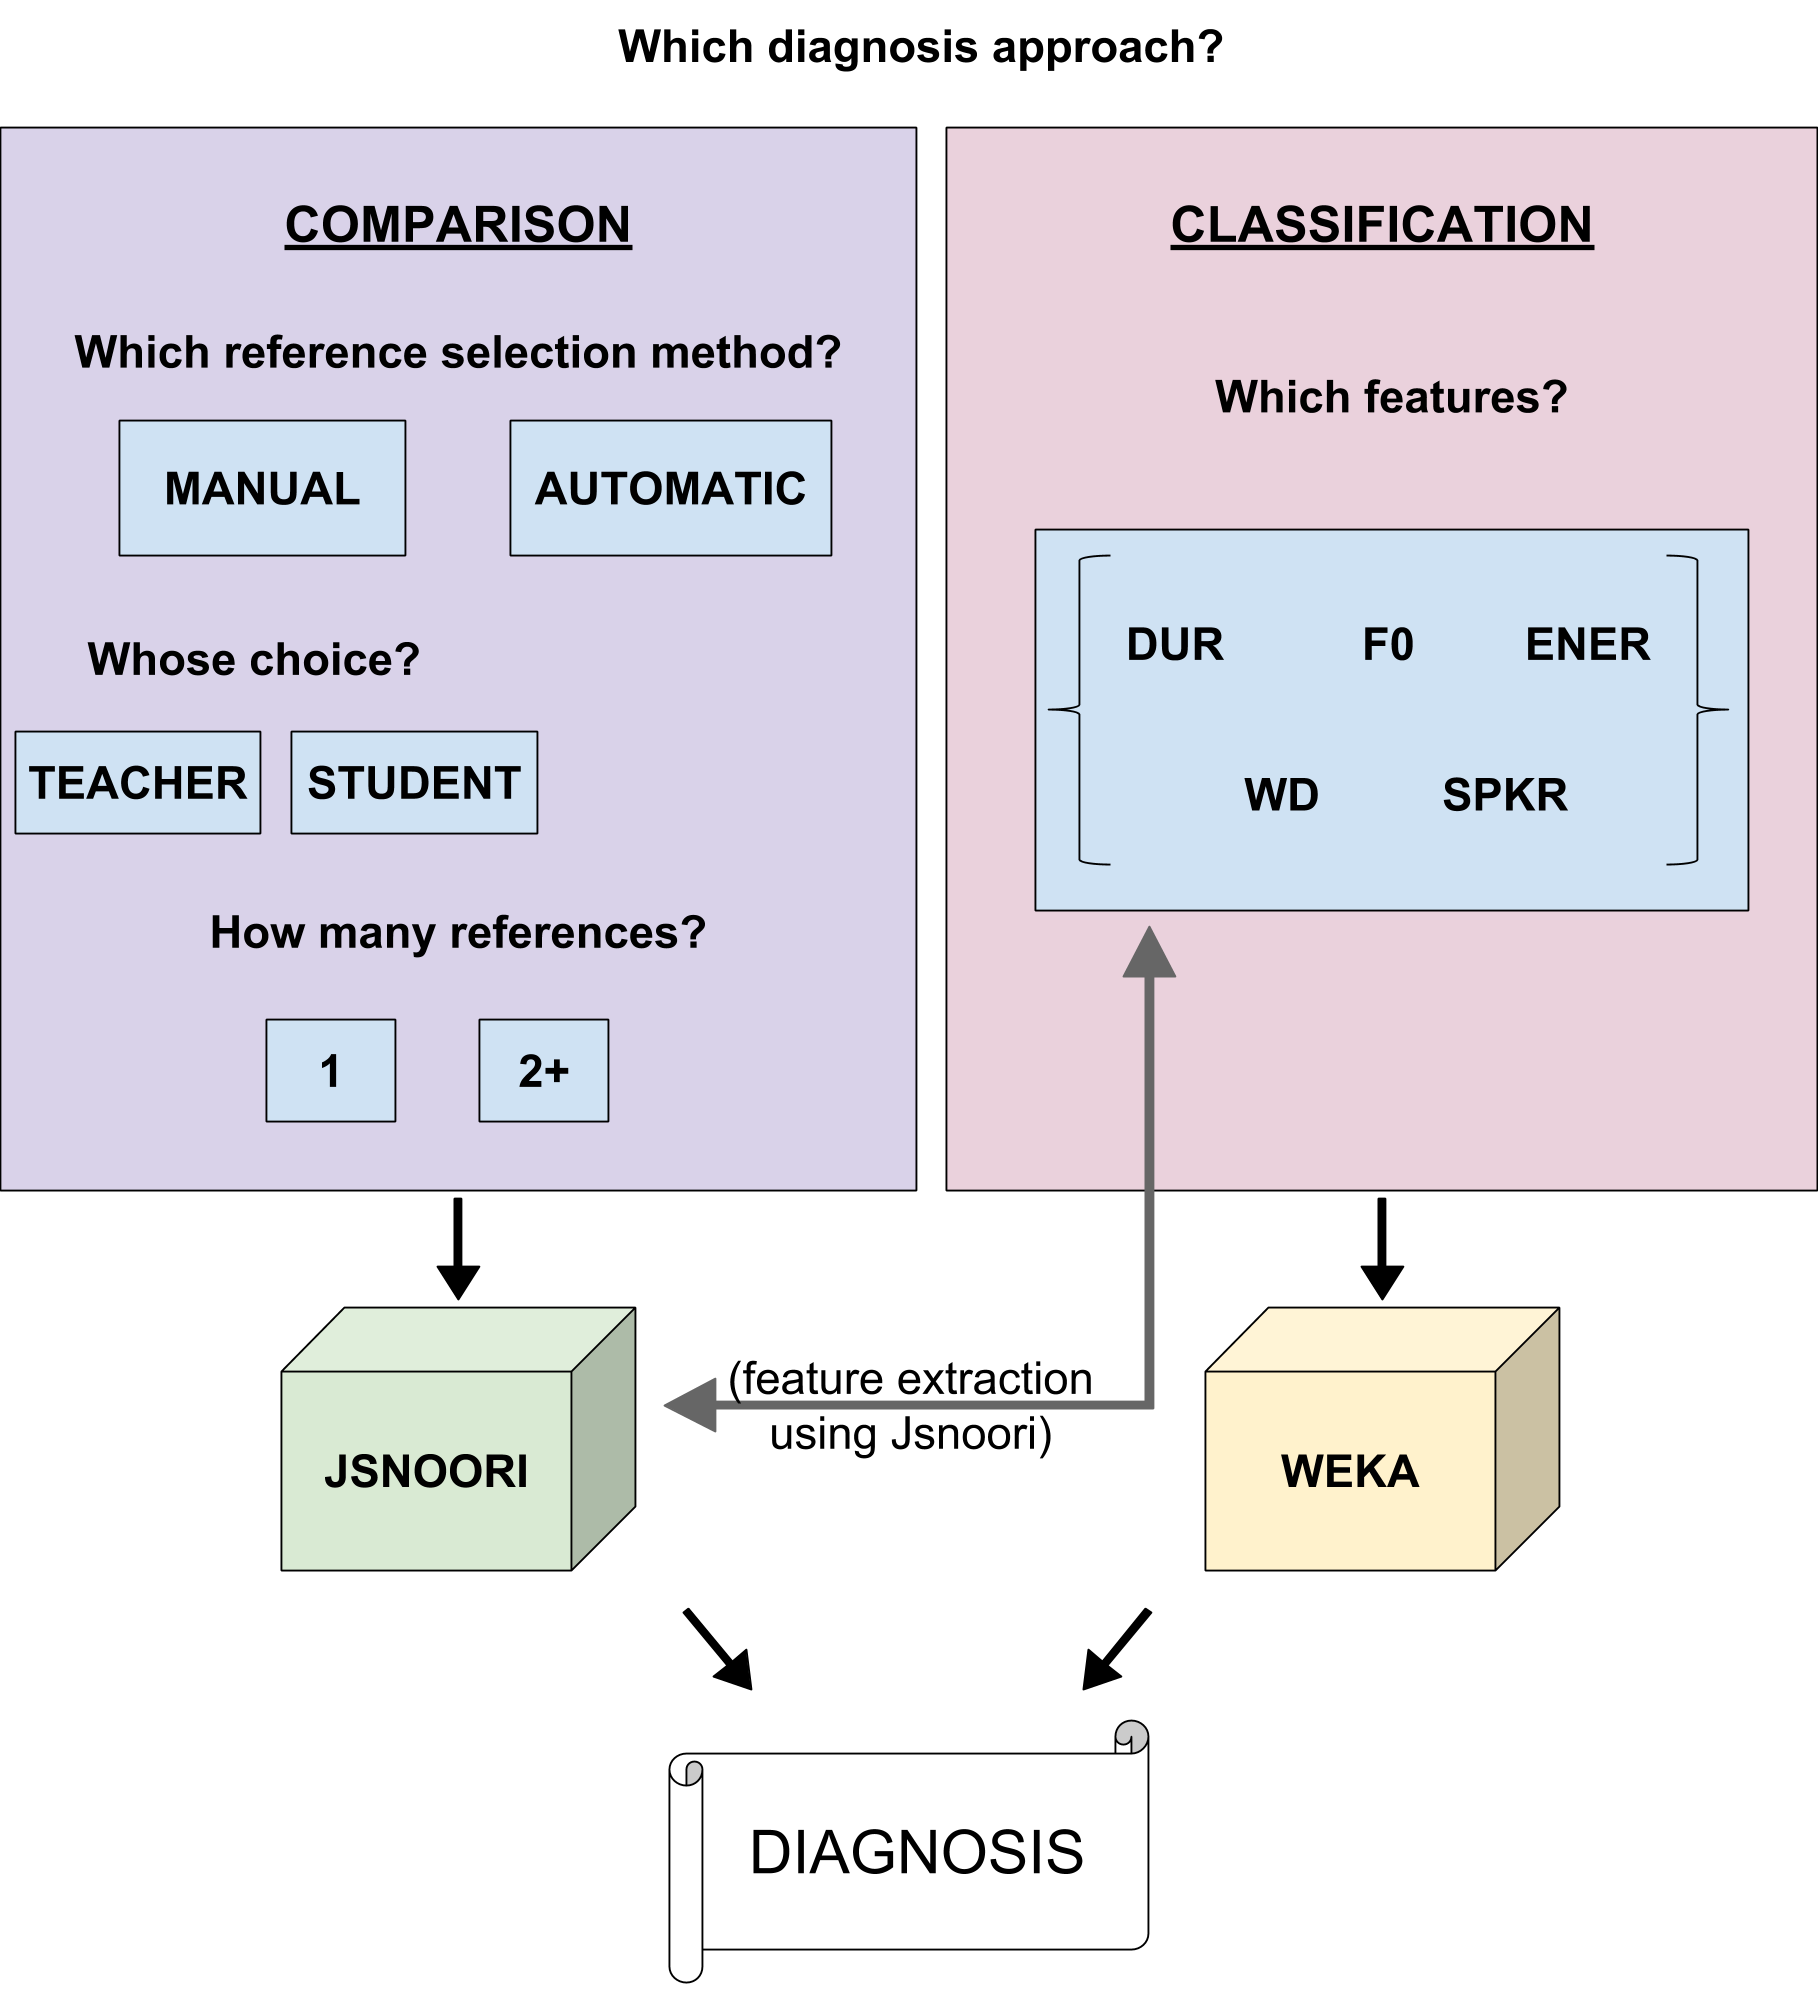
\includegraphics[width=\textwidth]{img/DiagnosisMethod}
		\label{fig:diag:system}
	\end{figure}
	
	\begin{figure}
		\centering
		\caption[Creating a DiagnosisMethod]{Screenshot of the researcher-facing interface to create a DiagnosisMethod}
		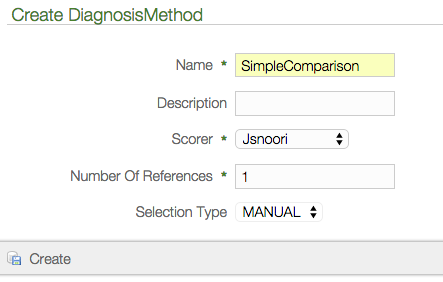
\includegraphics[width=.8\textwidth]{img/screenshots/createDiagnosisMethod}
		\label{fig:diag:creatediagnosismethod}
	\end{figure}
	
	
%	\begin{figure}
%		\centering
%		\caption[Creating an Exercise]{Screenshot of the researcher-facing interface to create an Exercise}
%		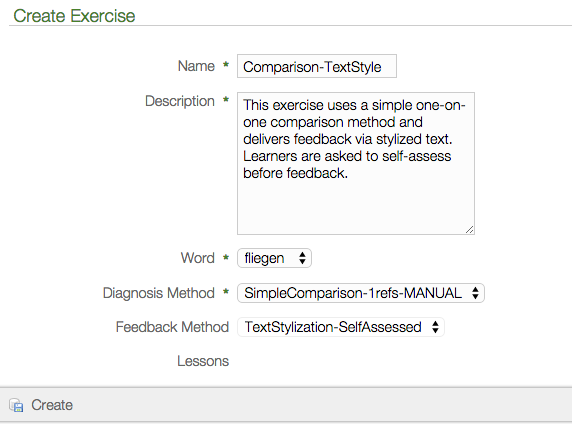
\includegraphics[width=\textwidth]{img/screenshots/createExercise}
%		\label{fig:diag:createexercise}
%	\end{figure}

\section{Summary}
\label{sec:diag:summary}


	This chapter has explored an array of methods by which lexical stress errors in the speech of French learners of German can be automatically diagnosed, as implemented in the modular diagnostic component of the \TODO{de-stress} CAPT tool.
	
	
	The first requirement for error diagnosis, accurate automatically-produced segmentations of the words, syllables, and phones of a learner's utterance (or that of a native speaker), can be obtained through forced alignment with the text of the utterance, as described in \cref{sec:diag:segmentation}. Forced alignment for German utterances being currently under development in the JSnoori software used by \TODO{de-stress} for speech processing, the current version of \TODO{de-stress} mocks this alignment step by using automatically-produced segmentations for utterances from the IFCASL corpus (\cite{Fauth2014,Trouvain2013}; see also \cref{sec:intro:ifcasl}).
	
	Analysis of the lexical stress realization of a given utterance, based on a set of prosodic features, is a second requirement for diagnosis, and \cref{sec:diag:prosody} has presented the set of features which can be used for such analysis in \TODO{de-stress}. These features capture the three acoustic properties most strongly correlated with the prosodic realization of lexical stress, namely duration, F0, and intensity. In \TODO{de-stress}, such features are extracted from a given utterance using the forced-alignment segmentations of that utterance and the speech processing capabilities of JSnoori.
	
	Using these features to represent a given L2 utterance as well as corresponding utterance(s) by L1 speakers, it is possible to assess the learner's utterance via one of two primary strategies: comparison or classification. \Cref{sec:diag:compare} has explored the possibilities for comparison-based diagnosis, in which features of the relevant segments of a learner's utterance are compared to the analogous features in a L1 utterance, and an error is diagnosed when the utterances differ considerably with respect to the relevant features. As described in \cref{sec:compare:single}, JSnoori uses this comparison-based approach to score each L2 utterance with respect to duration, F0, and prosody, and \TODO{de-stress} can use these scores as one form of diagnosis and a starting point for the delivery of certain types of feedback, as will be discussed in \cref{chap:feedback}. In addition to diagnosing an L2 utterance in comparison with a single L1 utterance, \TODO{de-stress} can combine scores with respect to multiple L1 utterances into a single score (see \cref{sec:compare:multi}), thus helping to reduce some of the risk of the diagnosis ``over-fitting'' to speaker- or utterance-dependent features of a single reference. Another option available in \TODO{de-stress} relates to the method of choosing the reference utterance(s) for a given learner utterance (see \cref{sec:compare:selection}); though many existing CAPT systems, including JSnoori, require manual selection of reference utterances, \TODO{de-stress} also offers an automatic selection option in which the reference is selected by choosing the L1 speaker(s) whose voice most closely resembles that of the learner in terms of F0 mean and range. 
	
	The second diagnosis strategy explored in this chapter (\cref{sec:diag:classification}), classification of lexical stress errors using machine learning algorithms, is a more novel approach to lexical stress error identification in CAPT, in which a learner's utterance is compared to the more abstract model of L1 speech represented by a classifier trained on a large number of L1 utterances. The experiments described in \cref{sec:classification:features,sec:classification:unseen} constitute original contributions to the understanding of how, and how effectively, classification-based diagnosis can be used to identify (in)correct realizations of lexical stress. As described in \cref{sec:classification:features}, the features seemingly most useful for classification relate to the duration and F0 of the utterance(s), unsurprising considering that these have been shown to be most closely linked to lexical stress in German \citep{Cutler2005,Dogil1999}. Features capturing the word type of the utterance as well as the age, gender and proficiency level of the speaker were also found to be quite valuable for error classification; combining these features with all three prosodic feature types resulted in the highest overall accuracy observed on this dataset (70.65\% accuracy, $\kappa=$0.31). As the observed agreement between the classifier's labels and the gold standard slightly exceeded the overall inter-annotator agreement observed when humans were asked to perform this error diagnosis task (see \cref{sec:lexstress:agreement}), these results seem encouraging. Unsurprisingly, slightly lower accuracy was observed when classifying utterances of word types or speakers not represented in the training data; however, the fact that accuracy on unseen words still remained comparable to the human inter-annotator agreement statistics seems to confirm the expectation that classification-based diagnosis may be a useful way to create CAPT systems which are are not limited to words/sentences for which recorded L1 utterances are available.
	
	
	While comparison-based diagnosis is not a new approach to identifying lexical stress errors in CAPT, the availability of multiple-reference comparison and automatic selection of reference speakers in the system, as well as the ability for researchers or instructors to configure the comparison method, make \TODO{de-stress} an important addition to the current CAPT landscape. The inclusion of a classification-based alternative to diagnosis is also a novelty for such a CAPT system, and this chapter's investigation of how L2 lexical stress errors can be diagnosed by classification is one of the major contributions of this thesis. By enabling researchers and instructors to choose among the various diagnosis options described in this chapter, \TODO{de-stress} will facilitate much needed future work exploring which diagnostic methods are most useful in which learning contexts, and which types of feedback (described in the following chapter) can best convey these diagnoses to the learner.